\documentclass[fleqn]{scrartcl}
\usepackage[ngerman]{babel}
\usepackage[T1]{fontenc}
\usepackage[utf8]{inputenc}
\usepackage[ngerman]{translator}
\usepackage{ae}
\usepackage{hyperref}
\usepackage{makeidx}
\usepackage{textcomp}
\usepackage{lmodern}
\usepackage{setspace}
\usepackage {amssymb}
\usepackage{graphicx}
\usepackage{listings}
\usepackage{fancyhdr}
\usepackage{pdfpages}
\usepackage{color}
\usepackage{paralist}
\usepackage{amsfonts}
\usepackage{amsmath}
%\usepackage{wasysym}
\usepackage{fancybox}
\usepackage{cancel}
\usepackage{graphicx}
\usepackage{algpseudocode}
\usepackage{algorithm}
\usepackage{algorithmicx}
\setcounter{tocdepth}{4}   %Aufnahme in das Inhaltsverzeichnis *
\setcounter{secnumdepth}{3}   %Nummerierung vertiefen *
\usepackage[b5paper, left=1.9cm, right=2.1cm, top=1.2cm, bottom=2.3cm]{geometry}


\title{Computerorientierte Mathematik}
\subtitle{Lernwissen zur Klausur}
\author{Stefan Hildebrand}
\date{\today}

%\makeindex

\begin{document}
\maketitle
\thispagestyle{empty}
\begin{center}
Wichtigste Quelle: 

Prof. Dr. Martin Skutella, Dr. Britta Peis: 

%\textbf{\large {}}
Vorlesungen der Computerorientierten Mathematik I und II

TU Berlin, WiSe 2012 - SoSe 2013
\end{center}
\vfill Berlin im September 2013 \hfill Geschrieben mit \LaTeX\\
Nachdruck nur mit Genehmigung der geistigen Urheber und des Verfassers!
%
%
\lstset{language=Java,
   basicstyle=\small,
   keywordstyle=\color{red},
   identifierstyle=,
   commentstyle=\color{blue},
   stringstyle= \color{green}\ttfamily,
   breaklines=true,
   numbers=left,
   numberstyle=\small,
   frame=single,
   backgroundcolor=\color{white}
}
%
\newpage
\tableofcontents
\newpage

%\pagenumbering{arabic}
\section{Kontrollstrukturen}
Die wichtigsten (zur Konstruktion der Turing- Maschine) sind:
\begin{itemize}
\item Zusammengesetzte Anweisungen\\
"Normaler Programmablauf": Werden sequentiell abgearbeitet.
\item bedingte Anweisungen\\
"$IF\, THEN\, ELSE\, ENDIF$": Stellen eine Entscheidung dar, von der nur eine abgearbeitet wird.
\item Schleifen\\
"$WHILE (Bedingung)\, DO\, ENDWHILE$": Anweisungsblock wird so lange abgearbeitet, bis die $Bedingung$ $false$ wird.\\
Ausformuliert als $WHILE, \,\, DO- WHILE\,\, und \,\, FOR(...)$ 
\end{itemize}
Alle Programmiersprachen, die diese 3 strukturellen Anweisungen kennen, sind gleich mächtig.
Es gibt aber auch äquivalente Alternativen (z.B. $goto$- Sprungbefehle).
In Java gibt es $goto$ zwar nicht, aber stattdessen $continue$ (springt sofort zum Schleifenanfang) und $break$ (beendet Schleife/ bedingten Anweisungsblock).

\subsection{Rekursion}
\subsubsection{Idee}
Um Rekursion zu verstehen, muss man erst Rekursion verstanden haben:

Ein rekursiver Methodenaufruf bedeutet, dass sich eine Methode selbst aufruft.
Dabei sollte (um ein Terminieren zu gewährleisten) entweder der übergebene Parameter bei jedem Durchlauf oder eine Klassenvariable, sozusagen der \glqq Zustand \grqq des Programms verändert werden.
Mathematisch: Eine Funktion wird (in Teilen) durch sich selbst definiert.

Selten ist eine Rekursion effizienter als eine Iteration, vor allem, wenn der Rekursionsbaum eine Liste darstellt (z.B. Endrekursion). Viele Probleme lassen sich dadurch jedoch eleganter und mit wesentlich weniger Programmieraufwand lösen, darüber hinaus ist Rekursion ein wichtiger Bestandteil des \glqq Divide- and Conquer \grqq- Prinzips.

Es gilt:\\
\begin{tabular} {c c c}
Anzahl rekursiver Aufrufe & $\widehat{=}$ & \# Knoten im Rekursionsbaum $ = T(n)$\\
Rekursionstiefe $ = h(n)$ & $\widehat{=}$ & Höhe des Stacks/ Aufrufbaums + 1
\end{tabular}

\subsubsection{Backtracking}
Wichtiger Problemlösungsansatz, basiert auf Trial and Error, gut rekursiv zu implementieren als eine Art Tiefensuche:\\

Wenn du dir irgendwo nicht sicher bist, probiere alle Möglichkeiten aus. Gibt es einen Fehler, nimm die letzte Änderung zurück und wähle eine andere Möglichkeit. Geht alles glatt, ist die Lösung korrekt.

\newpage
\section{Kodierung}
\subsection{Eindeutige Decodierbarkeit}
Ein Code heißt eindeutig decodierbar $\Leftrightarrow$ Verschiedene Original- Dateien führen zu verschiedenen codierten Dateien.

Eine injektive Codierung wird gefordert.
\subsection{Block- Code}
\begin{itemize}
\item Jedes Zeichen hat die selbe Länge in der Binär- Darstellung
\item Dadurch sehr einfache Kodierung und Dekodierung
\item Häufig verwendete Codierung
\item Beispiele sind ASCII, Unicode, etc.
\item Nachteil: \glqq Platzverschwendung \grqq
\end{itemize}
\subsection{Präfix- Code}
\begin{itemize}
\item Variable Länge: Zeichen \textit{können} unterschiedliche viele Bits in der Binär- Darstellung belegen.
\item \textit{Eine} wichtige Klasse von eindeutig decodierbaren Codes
\item Ein Code heißt Präfix- Code, wenn kein Codewort als Präfix eines anderen Codeworts auftaucht.
\item Jeder Blockcode ist ein Präfix- Code
\item Präfix- Codes lassen sich mit binären Bäumen identifizieren:

Ein Blatt im Baum entspricht einem Zeichen.\\
Zeichen $c \in C \leftrightarrow$ Weg im Baum von der Wurzel bis zum zugehörigen Blatt.\\
Die Kanten auf dem Weg geben die Bitfolge: 0 nach links, 1 nach rechts.

Dabei garantiert die Präfix- Code- Eigenschaft, dass Zeichen bei der Konstruktion des Baums nur in den Blättern auftauchen.
\end{itemize}

\newpage
\subsection{Datenkompression mit Huffman- Algorithmus}
\paragraph*{Idee} gängige Block- Codes (z.B. ASCII) umwandeln in Präfix- Code variabler Länge. Die kürzesten Präfix- Code- Zeichen werden für die häufigsten Block- Code- Zeichen benutzt.

Suche einen binären Baum T, dessen Blätter dem Zeichensatz C entsprechen und der die Größe $B(T) = \underset{c \in C}{\sum} f(C) \cdot h_T (c)$ minimiert, d.h. $B(T) \leq B(T') \forall$ Präfixcodes $T'$

\paragraph*{Algorithmus}$ $\\
\textbf{Input:} Ein Zeichensatz $C$, Häufigkeiten des Auftretens $f: C \rightarrow \mathbb{N}, c \mapsto f(c)$\\
\textbf{Output:} Ein optimaler Präfixcode als Huffman Baum
\begin{algorithmic}
\State Fasse jedes Zeichen $c \in C$ als einelementigen Baum auf und füge es in eine Priority Queue $Q$ ein, wobei die Häufigkeit $f(c)$ als Schlüsselwert dient.\\
\While {$Q$ enthält mehr als einen Baum}\\
\State Wähle die beiden Bäume $T_1$ und $T_2$ mit den kleinsten Häufigkeiten 
\State (muss nicht eindeutig sein).\\
\State Entferne sie aus $Q$.\\
\State Konstruiere einen neuen Baum aus den $T_1, T_2$ als Teilbäume 
\State unter einer neuen Wurzel und gebe ihm die Häufigkeit $f(T_1) + f(T_2)$.\\
\State Füge diesen Baum in $Q$ ein. \\
\EndWhile
\State \Return (Den einzig übrig gebliebenen Baum) $T$ in $Q$.\\
 Dieser Baum ist der Huffman Code/ Huffman Baum und ein optimaler Präfixcode.
\end{algorithmic}
\paragraph*{Bemerkungen zu Huffman- Codes}$ $\\\\
\begin{tabular}{l | l}
Huffman & alternativ\\
\hline
zeichenweise Codierung & nicht zeichenweise \\
 & (kodiere ganze Strings mit einem Code- Wort)\\
\hline
statische Kodierung & dynamisch: \glqq on the fly \grqq \\
Kodierung gilt für gesamte Datei,  & Codeworte werden beim Lesen \\
nach Häufigkeitsanalyse & der Datei erzeugt \\
 & und dynamisch verändert (\glqq adaptiv \grqq) \\
\hline
verlustfrei & verlustbehaftet
\end{tabular}
\newpage

\section{Datenstrukturen}
In Datenstrukturen können Daten in großer Menge und durchaus sortiert auftreten.

Sie alle haben 
\begin{itemize}
\item einen Wertebereich
\item Operationen
\item Komponenten- Daten (atomar oder selbst strukturiert)
\item Regeln, die das Zusammenwirken der Komponenten zur Struktur definieren
\end{itemize}

Lineare Strukturen haben darüber hinaus eine Ordnung, die eine erste und letzte Komponente sowie einen Vorgänger und Nachfolger für jede Komponente definiert.

Lineare Strukturen ermöglichen beliebigen Zugriff auf eine einzelne Komponente (random access), im Gegensatz zum sequentiellen Zugriff, bei dem vor der n-ten Komponente erst auf die n-1 ersten Komponenten zugegriffen werden muss.

Homogene Komponenten sind untereinander alle gleichartig (von gleichem Typ)

\subsection{Array}
Arrays sind besondere lineare Datenstrukturen. Sie kennzeichnet insbesondere:
\begin{itemize}
\item eine feste Komponentenzahl. Sie wird zur Laufzeit festgelegt.
\item der direkte Zugriff auf Komponenten per Indizes (vom Typ $int$).
\item ein homogener Grundtyp.
\item die Möglichkeit, Indizes zu berechnen
\item die Erzeugung einer ArrayIndexOutOfBoundsException, wenn der Index bei Zugriff nicht im gültigen Bereich liegt.
\item das einfache Durchlaufen per $for$- Schleife.
\end{itemize}
Dieses Konstrukt entspricht in der Mathematik einem Vektor.

\newpage
\subsection{Liste}
Dies ist keine lineare Datenstruktur. Hier hat jedes Datum seinen Nachfolger (und evtl. Vorgänger) selbst als Referenz abgespeichert. Bei Durchlaufen der Liste werden die Referenzen kopiert und so mit den Daten gearbeitet.

Auf der einen Seite ist kein random access möglich, stattdessen kann die Liste besonders schnell verlängert werden und Komponenten können sehr einfach eingefügt und entfernt werden.

Als Modell kann ein Seil aus zusammengeknoteten Fäden oder Bettlaken, (wie bei Gefängnisausbrüchen) dienen. Ein neues Stück lässt sich an einer bestimmten Stelle leicht anknoten, genauso wie sich ein Stück leicht entfernen lässt.

Operationen auf einer Liste:
\begin{itemize}
\item Erzeugung einer leeren Liste
\item Einfügen vor oder hinter einem Element
\item Löschen eines Elements
\item Prüfen, ob Liste leer ist
\item Test auf Ende der Liste
\item an den Anfang der Liste gehen
\item ein Element weiter gehen
\end{itemize}
\subsection{Stack}
Der Stack ist eine besondere Art Liste, bei der nur am Kopf zugegriffen werden kann (LIFO).
Er wird zum Beispiel als Runtime- Stack oder zum Finden von Paaren in einer Menge verwendet.

Die wichtigen Operationen lauten 
\begin{itemize}
\item push (Element hinzufügen)
\item peek (Element nur lesen)
\item pop (Element lesen und entfernen).

Anwendungsmöglichkeiten:
\begin{itemize}
\item Laufzeit- Stack in Java
\item Überprüfen korrekter Klammerung (Erkennen korrespondierender Klammernpaare)
\item Realisierung von Rekursion
\item Auswertung arithmetischer Ausdrücke
\item ...
\item außerhalb der Informatik: Rangierbahnhöfe
\end{itemize}
\end{itemize}
Anschauliche Darstellungen sind ein Stapel oder ein Kellerautomat, bzw. ein halb verstelltes Bücherregal.
\subsection{Queue}
Die Queue oder Schlange ist eine weitere spezielle Liste. Hier wird am Schwanz eingefügt, am Kopf gelesen und entfernt.

Die Schlange findet gerne Anwendung, um Wartezeiten zu verteilen, also als Warteschlange.
\subsection{Graphen}
Bestehen aus Knoten und gewichteten Kanten
\[V = Knotenmenge = \{1, ..., n\} bzw, \{0, ..., n-1\}\]
\[E = Kantenl"ange; E \subseteq \{{u, v}; u,v \in V\}\]
\subsubsection{Weg}
Der Weg in einem Graphen ist eine Folge von Kanten und eine Richtung pro Kante, sodass der Endpunkt einer Kante der Anfangspunkt der nachfolgenden Kante ist. Wiederholungen von Knoten und Kanten sind zulässig.

\subsubsection{Kantenbewertungen}
Pro Kante wird eine Zahl ("Entfernung") eingeführt. 
\subsubsection{Länge eines Weges}
Die Summe der Bewertungen der Kanten in der Folge. 
\subsubsection{Kürzester Weg von Knoten i zu Knoten j}
Der Weg mit der kürzesten Länge unter allen Wegen unter i nach j (es kann mehrere kürzeste Wege geben).

\subsubsection{Gerichtete (Di-) Graphen}
V, E bleiben gleich. Aber es werden gerichtete Kanten (Bögen) eingeführt.

Ein (endlicher) Digraph G besteht aus:
\[(endlicher) \quad Knotenmenge \quad V\]
\[Kantenmenge \quad E \subseteq V \times V \ \{(v, v) | v \in V\}\]
Schreibweise: $G = (V, E)$\\
Kantenbewertung: Funktion $w: E \rightarrow \mathbb{R}$

Nun werden Richtungen eingeführt, sodass der Durchlauf nur in einer Richtung möglich ist (wie auf Abbiegespuren, Einbahnstraßen). Der Begriff vom kürzesten Weg gilt entsprechend.

$\Rightarrow$ Ungerichtete Graphen können als Spezialfall von Digraphen gelten, die antiparallele Kanten haben, bzw. symmetrisch gerichtet sind. Somit reicht es aus, die Probleme nur für gerichtete Graphen zu diskutieren.

Achtung: Es sind auch negative Kantenbewertungen möglich.

\paragraph{Zykel}
Ein gerichteter Weg mit gleichem Anfangs- und Endknoten.

Enthält ein Weg zwischen i und j einen Zykel negativer Länge (negative Zykel), so gibt es keinen kürzesten Weg zwischen i und j.

Algorithmen liefern entweder den kürzesten Weg oder den negativen Zykel.
 
\subsubsection{Datenstrukturen für Digraphen}
\paragraph{Adjazenzliste}
Für jeden Knoten i gibt es eine Liste $Adj(i)$ der Knoten j, die Endpunkt einer Kante $(i, j)$ sind. Es ergibt sich ein Array von Listen, die man in einer Adjazenzmatrix zusammenfassen kann.

\paragraph{Adjazenzmatrix}
$A = (a_{ij})$ mit $a_{ij} = 1$, falls  $(i, j)$ Kante, 0 sonst.
\paragraph{Entfernungsmatrix}
$a_{ij} = $ Kantenbewertung, falls $(i, j)$ Kante; 0, falls $i = j$; $\infty$ sonst

\subsubsection{Bellman- Gleichungen}
$u_{ij}^{(m)} := $ Länge eines kürzesten Weges von i nach j mit höchstens m Kanten, falls dieser existiert; $\infty$ sonst\\\\
Bellman- Gleichung:
\[u_{ij} ^{(1)} = a{ij}\]
\[u_{ij}^{(m+1)} = \min_{k = 0, ..., n-1} [u_{ik}^{(m)} + a_{kj}] \quad \quad \text{für } m \geq 1\]

Es gilt das Prinzip der optimalen Teilstruktur: In einem kürzesten Weg sind alle Teilwege selbst kürzeste Wege.

\subsection{Bäume}
Spezieller Digraph, der genau einen Wurzelknoten hat.
Zu jedem anderen Knoten führt genau eine Kante und beliebig viele führen weg.
\subsubsection{voller binärer Baum:} Ein binärer Baum, bei dem alle Schichten (bis auf die letzte) voll besetzt sind. \glqq Jeder Knoten hängt so hoch wie möglich.\grqq\\
\textbf{\textit{vollständiger Baum:}} Jeder Knoten hat 0 oder 2 Kinder $\rightarrow$ Heap ist kein vollständiger Baum.

\subsection{Suchbäume}
\begin{itemize}
\item Verwaltet dynamische Daten
\item Unterstützt folgende 3 Operationen in $O (\log n)$:
\begin{itemize}
\item suchen
\item einfügen
\item löschen
\end{itemize}
\end{itemize}

Idee:
\begin{itemize}
\item binäre Bäume
\item Knoten eines Baumes $\widehat{=}$ Datensätze / Elemente mit Schlüsseln

\paragraph*{Suchbaumeigenschaft:}
Für jeden Knoten $v$ des Baumes haben alle Elemente im linken Teilbaum von $v$ einen kleineren Schlüssel als $v$, die Elemente im rechten Teilbaum einen größeren Schlüssel $\Leftrightarrow$ In Inorder- Traversierung sind die Schlüssel aufsteigend sortiert.
\end{itemize}

\subsubsection{Suchen}
\textbf{Input:} Suchbaum $T$, gesuchter Schlüssel $key$\\
\textbf{Output:} gesuchtes Element oder -1, falls Element nicht vorhanden
\begin{algorithmic}
\State Vergleiche gesuchten Schlüssel mit Schlüssel in Wurzel
\If {Gleichheit}
\State \Return Wurzelelement
\Else \If {$key$ < Root.key}
\State Suche rekursiv im linken Teilbaum weiter
\Else 
\State Suche rekursiv im rechten Teilbaum weiter
\EndIf
\EndIf
\State \Return -1
\end{algorithmic}
\paragraph*{Aufwand:} Suchen nach Knoten $v$ erfordert genau $h_T(v) + 1$ Vergleiche.

\subsubsection{Einfügen}
Idee: Suche nach einzufügendem Knoten, bis in Blatt angekommen. Erzeuge entsprechenden Kind- Knoten und hänge ihn auf der richtigen Seite an das Blatt an.
\paragraph*{Aufwand:} Wie Suchen $O (h(T))$ Vergleiche

\subsubsection{Löschen}
\begin{algorithmic}
\State Suche zu löschenden Knoten
\If {Knoten ist Blatt}
\State Blatt löschen, fertig.
\EndIf
\If {Knoten hat genau 1 Kind}
\State Ersetze Knoten durch sein Kind, fertig.
\EndIf
\If {Knoten $v$ hat genau 2 Kinder}
\State Suche im rechten Teilbaum von $v$ den linkesten Knoten $w$, d.h. mit kleinstem Schlüssel im Teilbaum
\State Vertausche Inhalte von $v$ und $w$
\State Lösche $w$, das kein linkes Kind hat.
\EndIf
\end{algorithmic}

Beachte: $w$ ist Nachfolger von $v$ beim Inorder- Durchlauf $\rightarrow$ Suchbaumeigenschaft bleibt erfüllt.

\paragraph*{Aufwand:} \begin{itemize}
\item Suchen von $v$ und $v$ in $O(h(T))$
\item Austauschen der Inhalte: $O(1)$
\item Löschen von $w$: $O(1)$
\end{itemize}
Insgesamt $O(h(T))$.

Alle 3 Operationen benötigen den Aufwand $O(h(T))$. Versuche also, Suchbäume mit spezieller Struktur zu verwenden, sodass $h(T) \in O(\log n)$.

\newpage
\subsubsection{Rotation}
\begin{figure*}[htbp]
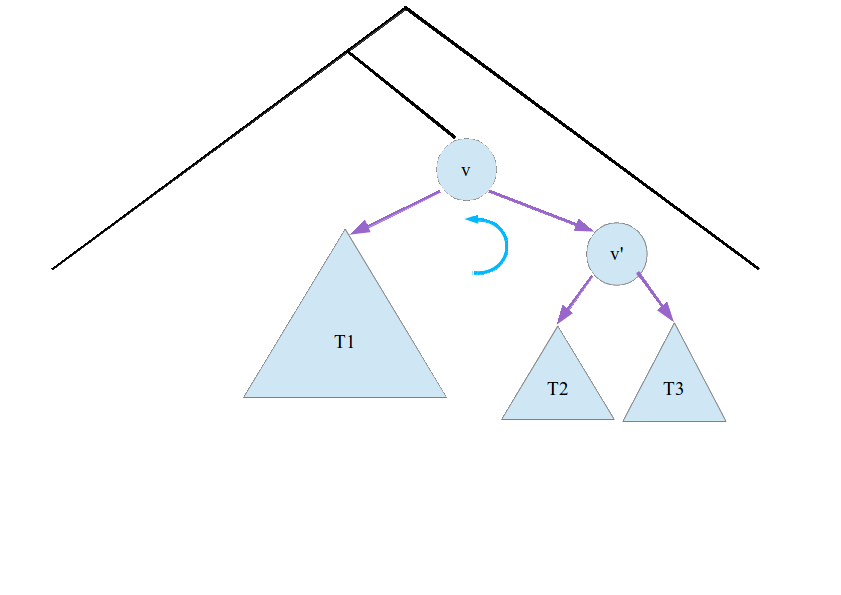
\includegraphics[scale=0.35]{./SuchbaumBaumRotieren1} \hfill
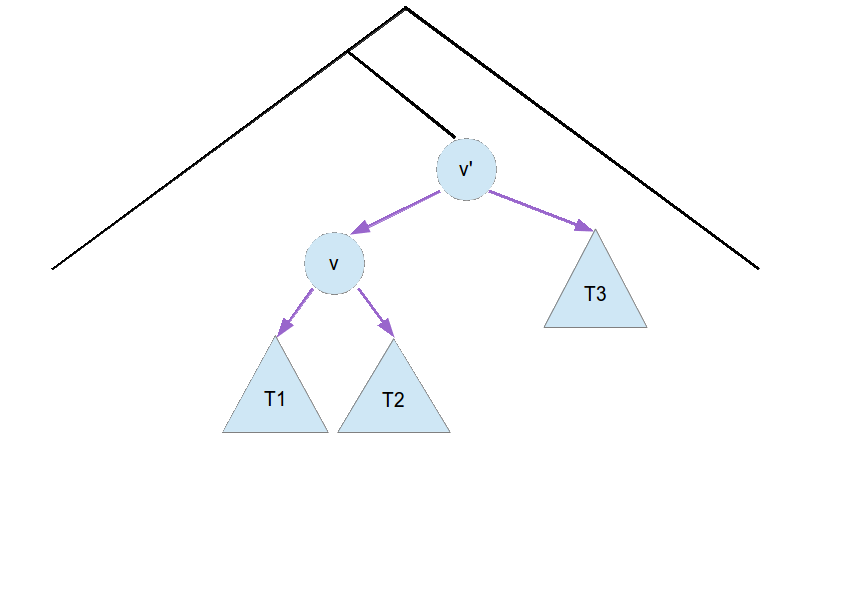
\includegraphics[scale=0.35]{./SuchbaumBaumRotieren2}
\end{figure*}
Rechtsrotation symmetrisch dazu und inverse Operation.

Beachte: Suchbaumeigenschaft bleibt erfüllt, denn 
\glqq $T_1 < v < T_2 < v' < T_3$ \grqq. Der Inorder- Durchlauf bleibt erhalten.

Links- und Rechtsrotation sind zusammen mächtig genug, um einen Suchbaum in jede gewünschte Gestalt zu bringen.
\paragraph*{Idee:} Bei dieser Operation wird der linke Teilbaum höher und der rechte weniger hoch.

\paragraph*{Aufwand:} Referenz auf $v$ gegeben, aktualisiere 3 Referenzen: $O(1)$

\subsubsection{AVL- Bäume}
Eine balancierte Klasse von Suchbäumen, die die folgenden Eigenschaften hat:
\begin{itemize}
\item[1.] Für jedes $n$ gibt es in der Klasse einen balancierten Suchbaum $T$ mit $h(T) \in O(\log n)$.
\item[2.] Die drei Basis- Operationen können auf dieser Klasse in $O(h(T))$ durchgeführt werden.
\item[3.] Die Klasse ist abgeschlossen unter den drei Basis- Operationen, d.h. nach Einfügen und/ oder Löschen eines Knotens muss der resultierende Baum wieder zu dieser Klasse gehören.
\end{itemize}

\paragraph{Definition Balance}
\[T \text{ binärer Suchbaum }, v \in V \text{ Knoten }, T_l(v), T_r(v) \text{ - evtl. leere Teilbäume von } v\]
\[\Rightarrow \beta (v) := h(T_r(v)) - h(T_l(v)), \quad h(\emptyset) = -1\]

\paragraph{Definition AVL- Baum} Ein binärer Suchbaum $T$ heißt AVL- Baum, falls für jeden Knoten $v$ in $T$ gilt:  $|\beta(v)| \leq 1$\\

Für einen AVL- Baum $T$ mit $n$ Knoten gilt: $h(T) \leq 2 \cdot \log(n)$

\paragraph{Idee des Beweises} Betrachte extremale AVL- Bäume, die zu vorgegebener Höhe eine minimale Anzahl Knoten enthalten.

\subparagraph{Definition} $T$ heißt extremaler AVL- Baum der Höhe $H$, falls $T$ AVL- Baum ist und $n(T) = \min\{n(T')\,\,|\,\,T' \,\, AVL- Baum, h(T') = h\}$

Vermutete Struktur eines extremalen AVL- Baums:
\begin{itemize}
\item[1] Höhendifferenz (Balance) ist in jedem inneren Knoten 1 oder -1.
\item[2] Für $h \geq 2$ sind $T_l$ und $T_r$ extremale AVL- Bäume zur Höhe $h-1$ und $h-2$
\end{itemize}
\subparagraph{Lemma} Ein extremaler AVL- Baum zur Höhe $h \geq 2$ hat als Teilbäume extremale AVL- Bäume zur Höhe $h-1$ und $h-2$.
\subparagraph{Beweis} Es sei $v$ Wurzel von $T$.

Falls $\beta(v) = 0$, dann kann man aus dem rechten Teilbaum alle Knoten auf dem Level $h$ löschen und erhält wieder einen AVL- Baum der Höhe $h$ mit weniger Knoten $\rightarrow$ \textbf{Widerspruch!}

$\Rightarrow$ Teilbäume $T_l$ und $T_r$ haben die Höhen $h-1$ und $h-2$.

Annahme: $T_l$ kein extremaler AVL- Baum zur Höhe $H(T_l)$.

Dann ersetze $T_l$ im Suchbaum $T$ durch extremalen AVL- Baum der Höhe $H(T_l)$. Dieser besitzt weniger Knoten, also besitzt $T$ nach dem Ersetzen weniger Knoten, ist aber weiterhin ein AVL- Baum zur Höhe $h \rightarrow$ \textbf{Widerspruch!}

Genauso: $T_r$ ist extremal.

Rekursionsformel für die Anzahl der Knoten eines extremalen AVL- Baumes:
\[n(h) = \left\{ \begin{array} {ll}
1 & h = 0\\
2 & h = 1\\
1 + n(h-1) + n(h-2) & h \geq 2
\end{array}\right.\]

\subparagraph{Lemma} Die minimale Knotenzahl $n(h)$ eines AVL- Baums der Höhe $h$ erfüllt:
\[n(h) \geq 2^{\frac{h}{2}}\]
\subparagraph{Beweis}
\begin{center}
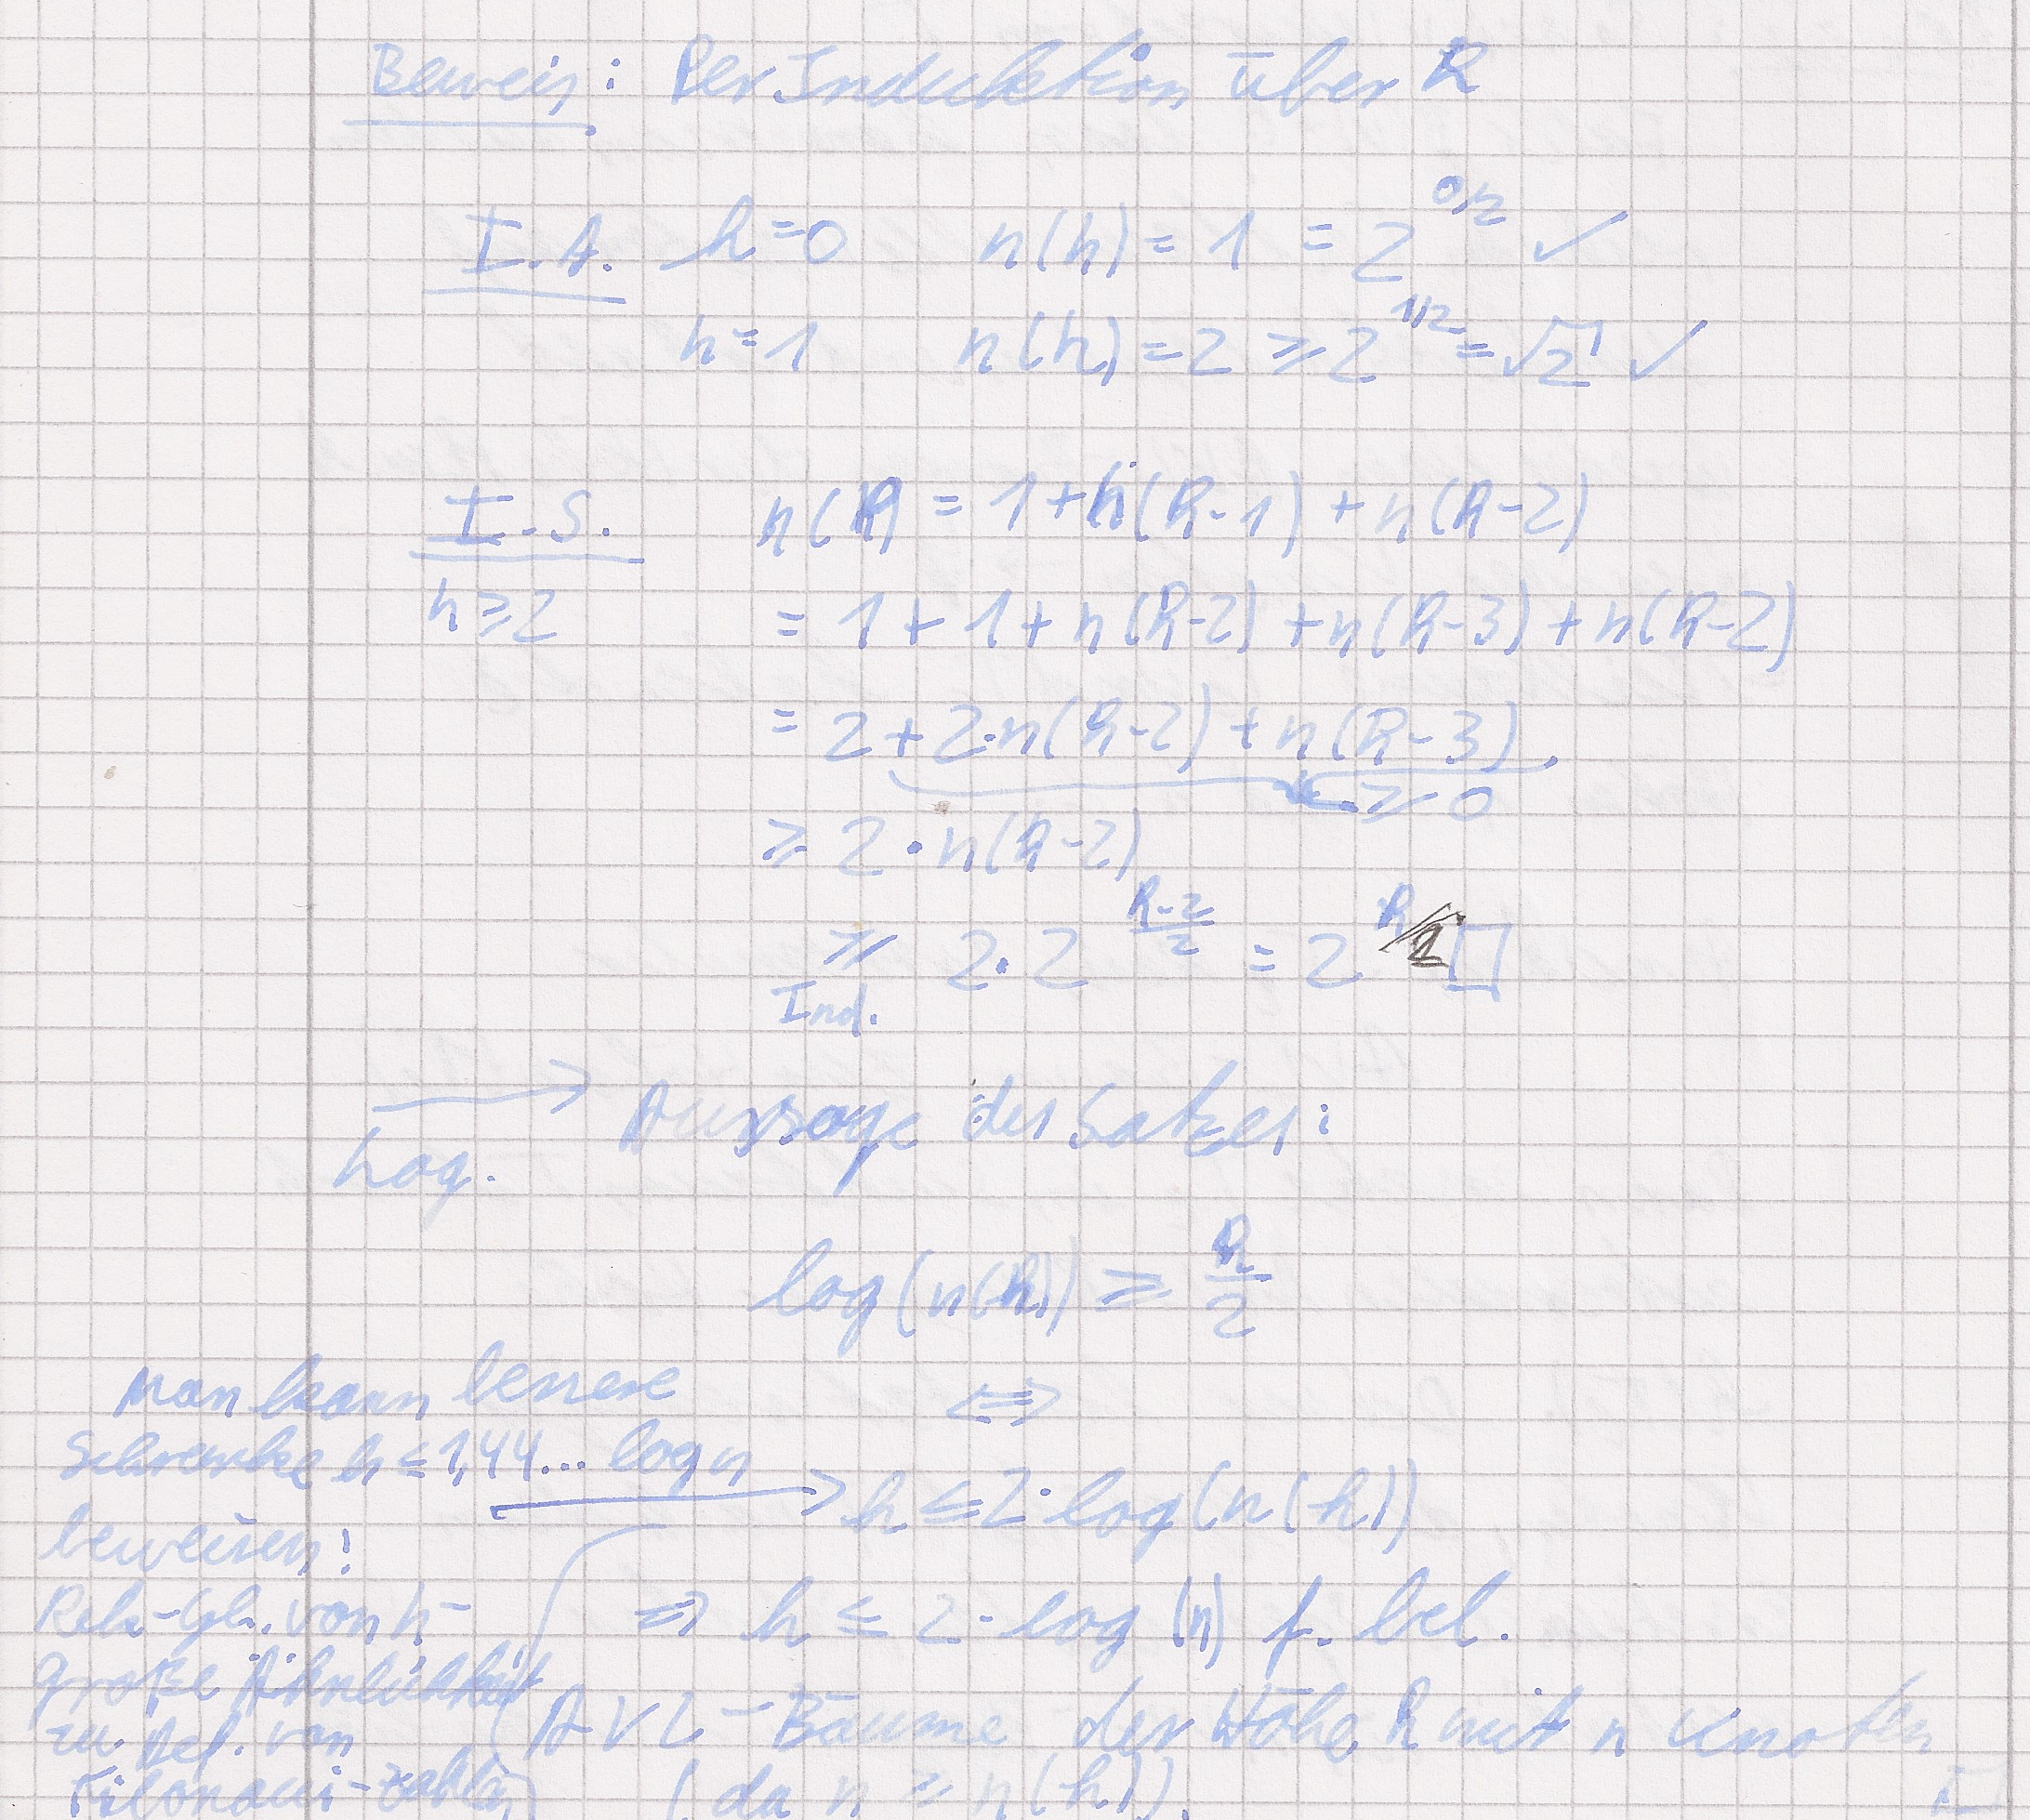
\includegraphics[width=\textwidth]{./extremaleAVLBaeume}
\end{center}

\newpage
\paragraph{Rotationslemma für AVL- Bäume}
Es gilt, falls $|\beta(v)| = 2$:
\begin{itemize}
\item[a] Rotation oder Doppelrotation: $T \rightarrow$ AVL- Baum, $h(T') \leq h(T)$
\item[b] Art der Rotation ist in $O(1)$ zu ermitteln.
\item[c] Rotation braucht $O(1)$- Aufwand.
\item[d] veränderte Balancen in $O(1)$ aus ursprünglichen zu berechnen.
\end{itemize}
4 Fälle in Abhängigkeit von den ersten beiden Kanten des Weges von der Wurzel v in die tiefste Tiefe des Baumes.

\begin{itemize}
\item[1.] Der Weg von $v$ in die größte Tiefe ist links- links.
\subitem Einfache Rechtsrotation \\
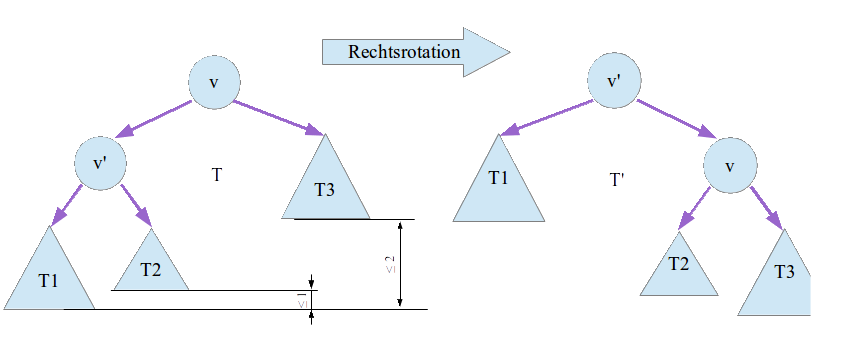
\includegraphics[width = \textwidth]{./Rechtsrotation}
\subitem Veränderte Situation in T':
\[\beta ' (v) = \left\{ \begin{array} {ll}
-1 & falls \beta(v') = 0\\
0 & falls \beta(v') = -1
\end{array}\right.\]
\[\beta ' (v') = \left\{ \begin{array} {ll}
1 & falls \beta(v') = 0\\
0 & falls \beta(v') = -1
\end{array}\right.\]
\[\beta ' (u) = \beta(u) \quad \forall \quad u \neq v, v'\]
\[h(T') = \left\{ \begin{array} {ll}
h(T) & falls \beta(v') = 0\\
h(T) -1 & falls \beta(v') = -1
\end{array}\right.\]
\newpage
\item[2.] Weg in die tiefste Tiefe geht links- rechts.
\subitem Links- Rechtsrotation \\
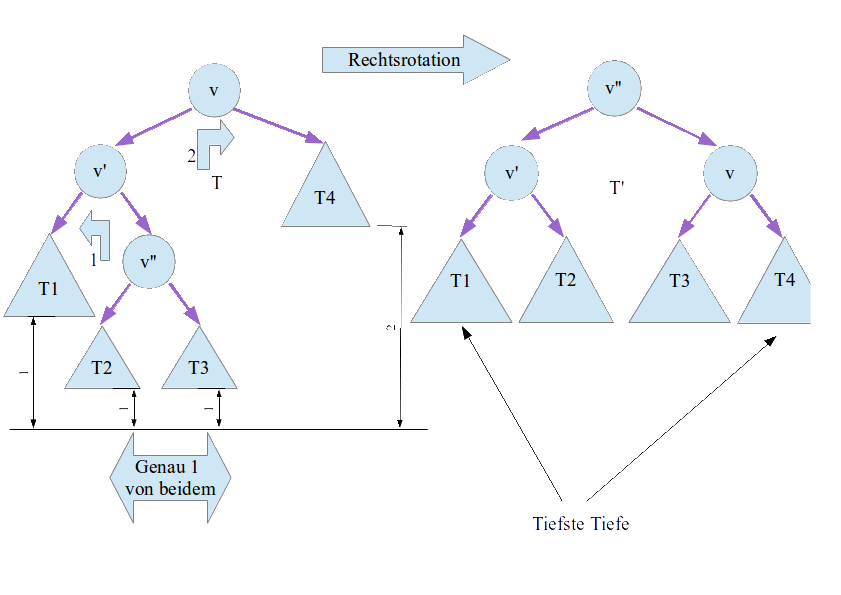
\includegraphics[width = \textwidth]{LinksRechtsrotation.png}
\begin{itemize}
\item $T_1$ verändert Tiefe nicht
\item $T_4$ rutscht 1 nach unten
\item $\Rightarrow$ beide liegen am Ende auf derselben Höhe.
\end{itemize}
\subitem Veränderte Situation in T':
\[\beta ' (v'') = \left\{ \begin{array} {ll}
0; & \beta(v'') = 0\\
0; & \beta(v'') = 1\\
0; & \beta (v'') = -1
\end{array}\right.\]
\[\beta ' (v') = \left\{ \begin{array} {ll}
0; & \beta(v'') = 0\\
-1; & \beta(v'') = 1\\
0; & \beta (v'') = -1
\end{array}\right.\]
\[\beta ' (v) = \left\{ \begin{array} {ll}
0; & \beta(v'') = 0\\
0 & \beta(v'') = 1\\
1; & \beta (v'') = -1
\end{array}\right.\]
\[\beta ' (u) = \beta(u) \quad \forall \quad u \neq v, v', v''\]
\[h(T') =h(T) -1 \]
\textbf{Beachte:} Berechnung der neuen Balancen in $T'$ und neue Höhe $h(T')$ in beiden Fällen in $O(1)$ zu berechnen.\\
\textbf{Bemerkung:} Falls der Weg in die tiefste Tiefe sowohl links- links, als auch links- rechts geht, so muss wie in Fall 1 verfahren werden, denn sonst reicht allein $T_1$ in die tiefste Tiefe und möglicherweise eins zu weit. Dann würde bei dem Fall des flachen $T_2$ gelten: $\beta(v') = -2$
\item[3.] Weg in die tiefste Tiefe beginnt rechts- rechts. $\rightarrow$ Analog zu 1. einfache Linksrotation.
\item[4.] Weg in die tiefste Tiefe beginnt rechts- links und \textit{nicht} rechts- rechts. $\rightarrow$ Analog zu 2. Doppel- Links- Rotation
\end{itemize}

\paragraph{Implementation der Basis- Operationen in AVL- Bäumen}
\subparagraph{Suchen:} Wie bei allgemeinen Suchbäumen mit Aufwand $O(h(T)) = O (\log n)$
\subparagraph{Einfügen:} Suche nach Schlüssel des neuen Elements endet erfolglos in einem Blatt. Hänge neues Element als linkes oder rechtes Kind an dieses Blatt an.\\
\textbf{Beachte:} Balancen haben sich höchstens auf dem Pfad von der Wurzel zum neuen Element geändert. $\rightarrow$ Gehe von neuem Element entlang der Spur zurück zur Wurzel und update und repariere die Balancen, falls nötig.

D.h. falls $\beta(v) \in \{-2; 2\}$ repariere dies sofort mit Rotationslemma.\\

\textbf{Aufwand:}
\begin{tabular} {l l}
Suchen & $O(\log n)$\\
Update \& Balance- Korrektur entlang Spur & $O (\log n)$
\end{tabular}\\\\
\textbf{Praktische Verbesserungsmöglichkeiten:}\\
Stellt man beim Verfolgen der Spur fest, dass sich die Tiefe des Teilbaums an einem Knoten $v$ nicht verändert hat, so kann man an dieser Stelle abbrechen.\\\\
Findet man beim Verfolgen der Spur nach oben einen Knoten $v$ mit $\beta(v) \in \{2; -2\}$ und behebt dies mithilfe des Rotationslemmas, so kann man danach stoppen, da die Höhe des Teilbaums an diesem Knoten wieder der Ausgangshöhe entspricht.

\textbf{Begründung:} Sei $v_1$ der erste gefundene Knoten mit $\beta(v_1) \in \{2; -2\} \rightarrow$ Höhe des TB an $v_1$ um 1 gewachsen durch Einfügen von $v$. Unterscheide symmetriebedingt folgende zwei Fälle:\\

\begin{tabular} {l l}
links- rechts- Weg: & Die Tiefe des Baumes schrumpft um 1 \\
links- links- Weg: & Bemerke, dass beide TB von $w$ die selbe Tiefe hatten,\\ & d.h. vor Einfügen von $v$ perfekt balanciert waren. \\ & Bei Rotation schrumpft die Tiefe \\& des TB an dem Knoten um 1.
\end{tabular}

\newpage
\subparagraph{Löschen}
\begin{itemize}
\item wie in allgemeinen Suchbäumen
\item aber: Balance möglicherweise verletzt $\rightarrow$ gehe daher entlang der Spur \\vom gelöschten Element zurück zur Wurzel, update Balancen, repariere ggf.
\item Aufwand: $O(\log n)$
\end{itemize}

\textbf{Bemerkung:} Leider gilt das schöne Resultat für das Einfügen \textit{nicht} für den Fall des Löschens, denn es gibt AVL- Bäume, bei denen nach dem Löschen eines Blattes an jedem Knoten der Spur das Rotationslemma angewendet werden muss.

Worst- Case- Beispiel: Lösche Blatt minimaler Tiefe in einem extremalen AVL- Baum.

\subsubsection{Optimale statische Suchbäume}
\begin{itemize}
\item Kenne alle Suchschlüssel $S = \{2_1, ..., s_2\}$
\item Kenne deren Zugriffshäufigkeiten $\beta_1, ..., \beta_n$, mit denen auf $s_1, .., s_n$ zugegriffen wird.
\item Beispiel: Daten auf CD
\item Ziel: Bestimme Suchbaum $T$ für $S$ und zu gegebenen $\beta_i$, sodass die mittlere Zugriffszeit klein ist.
\end{itemize}

Die Anzahl nötiger Vergleiche beim Suchen nach $s_i$ beträgt $h_T(s_i) + 1$.

Die mittlere Zugriffszeit ist:
\[E_p(T) = \frac{\sum\limits_{i = 1}^{n} \beta_i \cdot (h_T(s_i) + 1)}{\sum\limits_{i = 1}^{n} \beta_i}\]

Die konkreten Zugriffswahrscheinlichkeiten berechnen sich folgendermaßen:
\[p_i = \frac{\beta_i}{\sum\limits_{j = 1}^{n} \beta_j}\]

\paragraph{Ziel:} Finde Suchbaum $T$, sodass $E_p(T)$ minimal. Entwickle Algorithmus, der diesen $T$ findet.

$T$ ist optimaler statischer Suchbaum, falls $E_p(T) \leq E_p(T') \quad \forall \,\, T'$ Suchbäume $\Leftrightarrow \underbrace{\sum\limits_{i = 1}^{n} \beta_i (h_T(s_i) + 1)}_{:= c(T)} \leq \underbrace{\sum\limits_{i=1}^{n} \beta_i (h_{T'}(s_i) + 1)}_{= c(T')}$

Betrachte im Folgenden absolute Häufigkeiten $\beta_i$ statt $p_i$ und $c(T)$ statt $E_p(T)$.

\paragraph{Struktur von optimalen Suchbäumen}
Prinzip der optimalen Substruktur:

Sei $T$ Suchbaum für $S$, $T'$ Teilbaum von $T$.

$\Rightarrow$ Die Schlüsselmenge $S'$ der Schlüssel in $T'$ bildet konsekutive Teilsequenz (Intervall) $s_i < s_{i+1} < ... < s_j$ von $s_1 < s_2 < ... < s_n$.

\shadowbox{\begin{minipage}{0.95\textwidth}
\textbf{Beweis: \\}

Der Inorder- Durchlauf durch $T$ liefert die Schlüssel in $S$ in aufsteigender Sortierung (Sucbbaum- Eigenschaft). Dieser Durchlauf besucht die Knoten in einem Teilbaum $T'$ nacheinander ohne Unterbrechung durch Knoten außerhalb von $T'$.
\end{minipage}}

$\Rightarrow$ $T$ ist optimal für $S$ und $\beta_1, ..., \beta_n \Rightarrow T'$ optimal für $S' = \{s_i, s_{i-1}, ..., s_j\}$ und $\beta_i, \beta_{i+1}, ..., \beta_j$

\shadowbox{\begin{minipage}{0.95\textwidth}
$ $\\
\textbf{Beweis: \\}

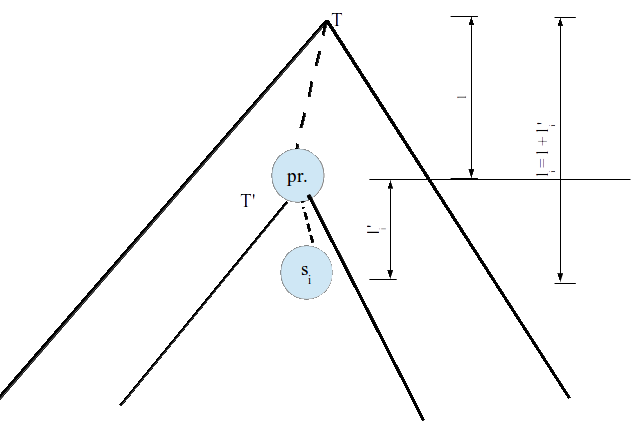
\includegraphics[scale=0.5]{optimalerSuchteilbaum.png}

\[l_i := h_T(s_i) + 1; \quad l_i' := h_{T'}(s_i) + 1; \quad l := h_T (s_k)\]
\[\Rightarrow l_i = l_i' + l\]
\[C(T) = \sum\limits_{q=1}^{n} \beta_q \cdot l_q = \underbrace{\sum\limits_{q=1}^{i-1} \beta_q \cdot l_q} _{V (\text{ vor } T')} + \sum\limits_{q=i}^{j} \beta_q \cdot l_q + \underbrace{\sum\limits_{q=j+1}^{n} \beta_q \cdot l_q}_{N (\text{ nach } T')}\]
\[= V + \sum\limits_{q=i}^{j} \beta_q (l + l_q') + N = \underbrace{V + N + \sum\limits_{q=i}^{j} \beta_q \cdot l}_{\text{Konstante unabhängig von }T'} + \underbrace{\sum\limits_{q=i}^{j}\beta_q \cdot l_q'}_{C(T') \text{, minimal } \Rightarrow C(T') \text{ minimal }} \] 
\[C(T') \leq C(T'') \quad \forall \quad \text{ Suchbäume } T'' \text{ für } s_i, ..., s_j; \beta_i , ..., \beta_j\]
Sonst wähle $\bar{T}$ mit $T''$ als Teilbaum statt $T'$. Dafür gilt
\[C(T) > C(\bar{T}), \text{ falls } C(T') > C(T'')\]
\end{minipage}}

Nutze die Einsicht: Falls $s_k$ Wurzel des optimalen statischen Suchbaums ist, dann sieht er so aus:
\begin{figure}[htbp]
\centering
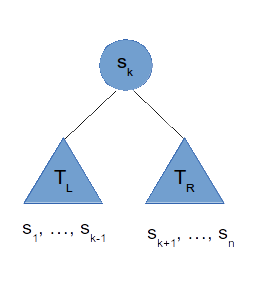
\includegraphics[scale=0.75]{optimalerSuchteilbaum2.png}
\end{figure}
Dabei ist \\
\begin{tabular} {l l}
$T_l$ opt. stat. SB f. & $s_1, ..., s_{k-1}; \beta_1, ..., \beta_{k-1}$\\
$T_r$ opt. stat. SB f. & $s_{k+1}, ..., s_n; \beta_{k+1}, ..., \beta_n$
\end{tabular}
Das heißt 
\[C (opt. \,\, SB) = \min_{h = 1, ..., n} \bigg[C(\text{opt. SB für } s_1, .., s_{k-1}) + C (\text{opt. SB für } s_{k+1} ..., s_n) + \sum\limits_{i = 1}^{n} \beta_i\bigg]\]
Für den Algorithmus bedeutet dies:
\begin{itemize}
\item Betrachte jede mögliche Wurzel $s_k, k = 1, ..., n$
\item Für diese Wurzel hänge optimale Teilbäume an
\item Wurzel auswählen, die $C$ minimiert.
\end{itemize}

Es sei $T_{ij}$ Suchbaum für $s_{i+1} , ..., s_j$. Wenn $T_{ij}$ die Wurzel $s_k$ hat, dann sind die Teilbäume $T_{i, k-1}$ und $T_{k, j}$.
Zugehörige Kosten: \[C(T_{ij}) =: C_{ij} = \beta_{i+1} \cdot l_{i+j}^{ij} + ... + \beta_j \cdot l_j^{ij} = \beta_{i+1} \cdot (l_{i+1}^{ij} - 1) + ... + 0 + \beta_j (l_j^{ij} - 1) + \underbrace{\sum\limits_{q = i+1}^{j}}_{W_{ij}} \beta_q\]
\[C_{ij} = C_{i, k-1} + C_{k, j} + W_{i j}\]

Wende Prinzip der optimalen Substruktur an:
\[C_{ij}^{opt} = \min_{i + 1 \leq k \leq j} \bigg(C_{i, k-1}^{opt} + C_{kj}^{opt} + W_{ij} \bigg) \]

Idee des Algorithmus': Berechne alle $C_{ij}^{opt}$ und zugehörige $T_{ij}^{opt}$ (optimale Teilbäume) nach aufsteigender Länge des Intervalls $i+1, .., j$.

Dieser Algorithmus ist Beispiel für das Prinzip der dynamischen Optimierung (Programmierung).

\paragraph{Aufwand:}
\begin{tabular} {l l l}
n & Bäume mit 1 Knoten & n\\
n-1 & Bäume mit 2 Knoten & n-1\\
n-2 & Bäume mit 3 Knoten & n-2\\
... & ... & ...\\
2 & n-1 & 2\\
1 & n & 1\\
\hline
Summe & & $\frac{n(n+1)}{2} \in O(n^2)$
\end{tabular}\\\\
Aufwand für die Berechnung eines dieser optimalen Teilbäume: $O(n)$ (Minimum über $n$ Terme)\\\\
\textbf{Gesamt:} $O(n^2 \cdot n) = O (n^3)$


\newpage\subsection{Priority Queue}
Ist eine dynamische Datenstruktur. Implementationsmöglichkeiten als
\begin{itemize}
\item Array (semi- dynamisch)
\item voller binärer Baum
\item sortierte Liste
\end{itemize}

Folgende Operationen werden unterstützt:
\paragraph*{Implementation als voller binärer Baum - Aufwand:} $ $\\
\begin{tabular} {c c c}
Operation & Name & Komplexität\\
\hline
Einfügen einer Komponente & insert() & $O (\log n)$\\
Zugriff auf Komponente mit größtem Schlüssel & max() & $O (1)$\\
Entferne Komponente mit größtem Schlüssel & extractMax() & $O (\log n)$\\
Ändern eines Schlüssels & changeKey & $O (\log n)$\\
\end{tabular}\\\\
Implementierungsdetails:
\begin{itemize}
\item Die Komponente mit größtem Schlüssel ist in der Wurzel.
\item $insert()$ - Hangle vom Zeiger $last$ auf letztes Blatt nach oben, bis Knoten linkes Kind ist. Gehe dann in rechten Ast, möglichst weit nach links und füge ein. Rufe dann $heapify()$ auf.
\end{itemize}
\paragraph*{Implementation als sortierte Liste - Aufwand:} $ $\\
\begin{tabular} {c c c}
Operation & Name & Komplexität \\
\hline
Einfügen einer Komponente & insert() & $O (n)$\\
Zugriff auf Komponente mit größtem Schlüssel & max() & $O(1)$\\
Entferne Komponente mit größtem Schlüssel & extractMax() & $O(1)$\\
Ändern eines Schlüssels & changeKey & $O(n)$\\
\end{tabular}

\subsection{Heap}
\begin{itemize}
\item spezielle Variante einer Priority Queue
\item homogener Komponententyp
\item alle Komponenten haben einen Schlüssel
\item Operationen wie Priority Queue als voller binärer Baum:
\end{itemize}

\paragraph*{Die Heap- Bedingung:}
Für jeden Knoten gilt: Die Schlüssel seiner Kinder sind kleiner als sein eigener. 

Implementierung als Array mit folgender Belegung: Die Kinder von Knoten $i$ haben die Indizes $2i + 1$ und $2i + 2$. Diese Implementierung eignet sich besonders für HeapSort, da dann keine weiteren Einträge hinzukommen können und auch dieses Sortierverfahren durch Umdefinieren der Array- Einträge ohne zusätzlichen Speicherplatz auskommt.

\subsubsection{Definition: Array als Heap}
Ein Array erfüllt die Heap- Eigenschaft $\Leftrightarrow$ Jeder Knoten in dem zugehörigen vollen binären Baum besitzt einen größeren Schlüssel als seine Kinder:
\[\forall \,\, i : vec[i].key > vec[2i + 1].key \land vec[i].key > vec[2i+2].key\]
für $(2i+1), (2i+2) > n$ (Länge des Arrays)

Dann gilt: \begin{itemize}
\item Größtes Element steht in vec[0]
\item Entlang eines Weges von der Wurzel zu einem Blatt können die Schlüssel nur (streng) monoton fallen.
\end{itemize}


\newpage
\section{Funktionen auf Datenstrukturen}
\subsection{auf Graphen}
\subsubsection{Bellman- Ford- Algorithmus}
Um die Matrix $U^{(n)}$ herzustellen, verwendet man Folgendes:
\[U^{(1)} = A\]
\[U^{(n+1)} = U^{(n)} \otimes A\]
Dabei ist die Bellman- Multiplikation so definiert:
\[A \otimes B = C \quad mit \quad c_{ij} = \min_{k = 1, ..., n} [a_{ik} + b_{kj}]\]

\begin{lstlisting}
public static double[][] bellman (double[][] a) {
	int n = a.length; //number of nodes
	double[][] u = new double[n][n];
	//initialize u
	for (int i = 0; i < n; i++)	{
		for (int j = 0; j < n; j++)
			u[i][j] = a[i][j];
	}
	for (int m = 2; m < n; m++)	{
	   	for (int i = 0; i < n; i++)		{
			double[] tmp = new double[n];
			//tmp array to calculate min[...] in 	
			//Bellman equation
			for (int j = 0; j < n; j++)
			{
				tmp[j] = u[i][j];
				for (int k = 0; k < n; k++)
				{
				   if (tmp[j] > u[i][k] + a[k][j])
					tmp[j] = u[i][k] + a[k][j];
					
				} //endfor k
			} //endfor j
			//store tmp in u[i]
			for (int j = 0; j < n; j++)
			{
				u[i][j] = tmp[j];
			}
		} //endfor i
	} //endfor m
	return u;
}
\end{lstlisting}

\paragraph*{Elementarer Zykel}
Ein Zykel, in dem jeder beteiligte Knoten genau ein mal besucht wird (außer dem Anfangs- und Endknoten, der wird genau zwei mal besucht).

\subsubsection{Ermittlung negativer Zykel} $ $
\textbf{Satz:}
G hat einen negative Zykel $\Leftrightarrow$ G hat einen \textit{elementaren} negativen Zykel $\Leftrightarrow$ Es gibt einen Knoten i mit $u_{ii}^{(n)} < 0$.

Somit wird die Existenz negativer Zykel mit einer zusätzlichen Iteration $(m = n)$ und Überprüfung der Diagonalelemente festgestellt. Alternativ kann man auch eine Änderung der Matrix während der letzten Iteration überprüfen.

\subsubsection{Floyd- Warshall- Algorithmus}
\textbf{Idee:} $dist(v, w, X) := $ Länge eines kürzesten v- w- Weges, der nur Knoten aus $\{ v, w\} \cup X$ besucht. 

Es wird definiert:
\[dist (v, w, \empty) := a_{vw}\]
\[dist (v, w, \{X\}) := \min \bigg[dist(v, w, \empty), dist (v, x, \empty) + dist (x, w, \empty) \bigg] \]
Ein erlaubter Zwischenstopp oder ohne Zwischenstopp
\[dist (v, w, \{x_1, ..., x_k \})\]
\[= \min \bigg[ dist(v, w, \{x_1, ..., x_{k-1} \}), dist(v, x_k, \{x_1, ..., x_{k-1} \} ) + dist(x_k, w, \{x_1, ..., x_{k-1}\})\bigg]\]

Entweder bekannte Wege oder ein neuer Umweg $\Rightarrow$ Rückführung auf den Fall mit einem Zwischenstopp weniger.

\paragraph{Pseudocode} 
\textbf{Input:} Adjazenzmatrix A
\textbf{Output:} Distanzmatrix Dist
\begin{algorithmic}
\For {(v = 0, ..., n-1)}
\For {(w = 0, ..., n-1)}
\State $dist (v, w, \emptyset ) := a_{vw}$ \Comment {(Initialisieren)}
\EndFor
\EndFor
\For {(i = 1, ..., n-1)}
\For {(v = 0, ..., n-1)}
\For {(w = 0, ..., n-1)}
\State  $dist (v, w, \{0, ..., i\}) := \min \bigg[ dist(v, w, \{0, ..., i-1\}), dist (v, i, \{0, ..., i-1\}) + dist(i, w, \{0, ..., i-1\})\bigg]$
\EndFor
\EndFor
\EndFor
\end{algorithmic}
$ $\\
\textbf{Laufzeit:} $O(n^{3})$\\
\textbf{Laufzeit von Bellman- Ford:} $O (n^{3} log (n))$ bzw. $O (n^{4})$

\paragraph{Tree- Matrix}
$tree_{ij} :=$ Vorgängerknoten von j auf dem i-j-Weg

Initialisierung: $tre_{ij} = $ i, falls $(i, j) \in E$; -1, sonst

Updates um Bellman- Ford- Algorithmus:
\begin{lstlisting}
for (int k = 0; k < n; k++)
{
	if (u[i][j] > u[i][k] + a[k][j])
	{
		u[i][j] = u[i][k] + a[k][j];
		tree[i][j] = k;
	}
}
\end{lstlisting}
$\Rightarrow$ Für jeden Startknoten v lässt sich aus $tree[v]$ ein Kürzester- Wege- Baum basteln.

\paragraph{Adjazenzlisten}
\textbf{Idee:} Platz sparen.

\textbf{Umsetzung:} Jeder Knoten erhält eine Liste seiner Nachbarn.

\textbf{Vorteile:} Schneller bei dünnen Graphen, wenn Algorithmen die Nachbarn eines Knoten oder alle Knoten suchen. Spart Speicher

\textbf{Nachteile:} Bei dichten Graphen speicherhungriger durch Overhead; Suche nach einer speziellen Kante im Graphen dauert länger.

\subsubsection{Tiefensuche im Graphen}
\begin{algorithmic}
\State Erzeuge einen Stack, packe Knoten s darauf.
\While {(Stack ist nicht leer)}
\If {(oberster Knoten n weiß)}
\State n orange färben, seine weißen Nachbarn auf den Stack legen
\ElsIf {(n orange)}
\State n rot färben, vom Stack entfernen
\ElsIf {(n rot)}
\State n vom Stack nehmen
\EndIf
\EndWhile
\end{algorithmic}
$ $\\
\textbf{Mittels Rekursion, ohne einzelnen Stack:}
\begin{algorithmic}
\State Färbe alle Knoten weiß
\State Rufe Tiefensuche für den Startknoten s auf
\end{algorithmic}
\textit{Tiefensuche- Methode für einen Knoten v:}
\begin{algorithmic}
\State Färbe v orange
\State Rufe für jeden weißen Nachbaren w die Tiefensuche- Methode auf
\State Färbe v rot
\end{algorithmic}

$ $\\
\textbf{Laufzeit:} jede Kante wird genau einmal betrachtet\\
\textbf{Speicherbedarf:} pro Kante wird maximal 1 Knoten auf den Stack gelegt

$\Rightarrow$ Die Laufzeit ist linear von der Anzahl der Kanten abhängig.\\
\textbf{Einsatzmöglichkeiten:} Gerichtete Zykel entfernen, alle Knoten durchsuchen, ...

\subsubsection{Breitensuche}
\begin{itemize}
\item wendet Queues an
\item traversiert einen Graphen
\item Berechnet kürzeste Wege in ungewichteten Graphen
\end{itemize}

Ideen:
\begin{itemize}
\item Beginne bei Startknoten
\item Benutze Adjazenzlisten, um neue Knoten zu finden
\item Markiere Knoten:
\subitem Weiß für noch nicht besuchte Knoten
\subitem Orange für besuchte Knoten, von denen weitergesucht wird
\subitem Rot für besuchte Knoten, von denen nicht weitergesucht wird
\item Benutze zwei Queues, um Knoten der aktuellen Phase und Knoten der nächsten Phase zu merken
\item Nummeriere der Knoten nach der Phase, in der sie bearbeitet werden ($\rightarrow$ Distanz)
\end{itemize}

Basisalgorithmus mit Startknoten s:
\begin{itemize}
\item Färbe alle Knoten weiß
\item Erzeuge zwei leere Queues
\item Füge s in die zweite Queue ein
\end{itemize}
\begin{algorithmic}
\While {zweite Queue nicht leer}
\State Verschiebe die Knoten der zweiten Queue in die erste Queue
\State Nächste Phase beginnt
\While {erste Queue nicht leer}
\State Betrachte den ersten Knoten v der ersten Queue
\State Färbe den Knoten rot und gib ihm die aktuelle Phasennummer
\State Weiße Nachbarn werden orange und zur zweiten Queue hinzugefügt
\EndWhile
\EndWhile
\end{algorithmic}

\subsection{Suchalgorithmen auf linearen Datenstrukturen}
\subsubsection{Sequentielle Suche}
Gegeben: Feld a, Wert x\\
Gesucht: Index k mit a[k] = x; Falls $\nexists$-1\\\\
Durchlaufe Feld von a[0] bis a[n-1] der Reihe nach.\\
Falls a[k] = x, gib k zurück\\
Ist a[n-1] $\neq$ x, gib -1 zurück.\\
\\
Aufwand: Im worst Case: n-1
\subsubsection{Binäre Suche} $ $\\
Feld ist sortiert, d.h. a[0] < a[1] < ... < a[n-1].\\
Finde Index k mit a[k] = x. Sonst gib -1 zurück.\\
\\
Wähle mittleren Index k und vergleiche x und a[k].\\
Ist a[k] = x, gib k zurück.\\
Ist x < a[k], so suche im Teilfeld a[0] ... a[k-1].\\
Ist a[k] < x, suche im Teilfeld a[k+1] ... a[n-1].\\
Verfahre so weiter, bis x gefunden. Ist der noch zu durchsuchende Teil leer, gib 1- aus.\\
\\
Aufwand: $C(n) \leq \lfloor \log n \rfloor +1$
\subsection{Sortieralgorithmen}
\subsubsection{Bubble Sort}
\begin{algorithmic}
\For {(i := 1 to n -1)}
\For {(j := 1 to n-1)}
\If {(a[j].key > a[j+1].key)}
\State vertausche (a[j], a[j+1])
\EndIf
\EndFor
\EndFor
\State \Return a
\end{algorithmic}

\subsubsection{SelectionSort}
\begin{algorithmic}
\For {(i := 1 to n-1)}
\State min := i
\For {(j := i+1 to n)}
\If {(a[j].key < a[min].key)}
\State min := j
\EndIf
\EndFor
\State vertausche (a[i], a[min])
\EndFor
\State \Return a
\end{algorithmic}
\subsubsection{InsertionSort}
\begin{algorithmic}
\For {(i := 1 to n-1)}
\State temp := a[i]
\State j:= i-1
\While {(j > 0 $\land$ a[j].key > temp.key)}
\State vertausche (a[j], a[j+1])
\State j := j-1
\EndWhile
\EndFor
\State \Return a
\end{algorithmic}
\subsubsection{MergeSort}
\begin{algorithmic}
\If {(n = 1)}
\State \Return a
\EndIf
\State a1 := firstHalf (a)
\State a2 := secondHalf (a)
\State a1 := MergeSort (a1)
\State a2 := MergeSort (a2)
\State a := merge (a1, a2)
\State \Return a
\end{algorithmic}
\subsubsection{QuickSort}
\begin{algorithmic}
\If {(n = 1)}
\State \Return a
\EndIf
\State p := a[n/2]
\State a1  $:= QuickSort(\{a[i] \, |\, a[i] \leq p\})$
\State a2 $:= QuickSort(\{a[i] \, |\, a[i] \geq p\})$
\State a := {a1, a2}
\State \Return a
\end{algorithmic}
Anmerkung: im Average Case $O (n \log n)$,\\ im Worst Case (Pivotelement stets das Maximum oder Minimum) $O (n^{2})$.\\ Praktisch der schnellste.

\subsubsection{HeapSort}
\paragraph{Algorithmus zur Herstellung der Heap- Eigenschaft} $ $\\
\textbf{Input:} (Item[] vec, int top, int bottom)\\
\textbf{Output:} Array Item[] vec, das die Heap- Eigenschaft erfüllt
\begin{itemize}
\item[] Setze voraus, dass Heap- Eigenschaft im Teilarray von $top + 1$ bis $bottom$ bereits erfüllt ist.
\item[] Stelle dann sicher, dass Heap- Eigenschaft erfüllt ist von $top$ bis $bottom$.
\begin{itemize}
\item[1)] Ermittle das größere der beiden Kinder von $top$ (falls Kinder im Teilarray existieren), nenne es child.
\item[2)] Vergleiche vec[top].key mit vec[child.key]
\subitem IF (vec[top].key > vec[child])
\subsubitem$\rightarrow$ Fertig! (RETURN)
\subitem ELSE
\subsubitem$\rightarrow$ Vertausche Komponenten von $top$ und $child$
\item[3)] Wende heapify rekursiv auf den Bereich von $child$ bis $bottom$ an.
\end{itemize}
\end{itemize}

Die Heapeigenschaft eines Arrays kann durch wiederholtes Aufrufen dieser Methode mit einer Laufzeit in $O (n)$ hergestellt werden.

\paragraph{Der eigentliche Sortiervorgang}
Tausche im ersten Durchlauf das größte Element an die letzte Stelle des Arrays, im zweiten Schritt das zweitgrößte an die vorletzte, usw.\\
\textbf{Aufwand:} $O(n) + n$ Aufrufe von heapify für Element an der Stelle 0 $\leq O(n) + n \cdot O(h) \in O (n \log n)$

\subsubsection{Untere Komplexitätsschranken für das Sortieren}
Es wurde gezeigt, dass jedes Sortierverfahren, das auf paarweisen Vergleichen beruht, im worst case wie auch im average case mindestens $\Omega (n \log n)$ Vergleiche benötigt.

Beweisidee: Im Entscheidungsbaum, den ein solcher Algorithmus zwangsweise abläuft, sind die tiefsten Blätter sowie der Höhendurchschnitt der $n!$ Blätter in einer Höhe von $\Omega (n \log n)$ zu finden.

\newpage
\subsubsection{BucketSort}
Ziel ist keine lineare Auflistung, sondern das Einsortieren der Einträge in der Eingabe (Liste, Array, etc.) in "Kategorien" (Listen, Queues), sodass in manchen Kategorien mehrere Einträge auftreten können, in anderen gar keine. Als Veranschaulichung: Ein Briefträger sortiert die Briefe einer Straße nach Hausnummern.\\\\
\textbf{Input:} $n$ Objekte $a_1, ..., a_n$ (Liste mit Schlüsseln), wobei die Schlüssel $s(a_1), ..., s(a_n) \in \{0, ..., m-1\}$\\
\textbf{Output:} Eine Liste, die an Stelle $i$ alle Objekte mit dem Schlüssel $i$ in einer gesonderten Liste enthält.
\paragraph{Aufwand:}
$O(n+m)$ Insbesondere, falls $m \leq n$, $m \in O(n) \Rightarrow$ Aufwand liegt in $O(n)$.

\subsection{Hashing}
\begin{itemize}
\item gestreute Speicherung
\item Alternative zu Suchbäumen
\item Unterstützt
\begin{itemize}
\item Suchen
\item Einfügen
\item Löschen (partiell)
\end{itemize}
\item Vorteil: Aufwand pro Operation im Mittel $O(1)$
\item Nachteil: Im Worst Case Aufwand $O(n)$
\end{itemize}



\subsubsection{Grundidee}
\begin{itemize}
\item Reserviere Hashtabelle mit $m$ Plätzen im Speicher, in der die abgespeicherten Daten stehen (ähnlich einem Array).
\item Gegeben: Datensätze mit Schlüssel, die aus Universum $U$ stammen.
\item Man kennt aber a priori nicht die Schlüssel der n Datensätze. Ganz $U$ kommt in Frage
\item $n := \# \text{ Datensätze in Teilmenge } << |U|$
\item Die Hashfunktion berechnet die Speicheradresse aus dem Schlüssel:
\subitem $h: U \rightarrow \{0, 1, ..., m-1\}$
\item Hier: Schlüssel $k$ sind ganze Zahlen
\end{itemize}

\paragraph*{Zur Umsetzung}
\begin{itemize}
\item Einfachste Lösung (\glqq direct addressing \grqq): $h$ bijektive Abbildung.\\
Belegt aber viel mehr Speicher als nötig, falls $U$ deutlich größer als die interessante Teilmenge.
\item Ziel: Größe der Hashtabelle soll ungefähr Anzahl der Datensätze entsprechen.
\item Es gilt i.A.: $h$ nicht injektiv, da $|U| > m$
\item i.A. $\exists k_1 \neq k_2$ mit $h(k_1) = h(k_2)$, d.h. Kollision
\item Kollision tritt fast sicher auf, kaum zu vermeiden. Hashverfahren muss mit Kollisionen umgehen können
\end{itemize}

\subsubsection{Kriterium für eine gute Hash- Funktion}
$h$ streut gleichmäßig über den Adressraum:
Jede Adresse wird mit der gleichen Wahrscheinlichkeit $\frac{1}{m}$ gewählt (\glqq uniform hashing\grqq).\\
In der Praxis nur angenähert zu realisieren.
Nutze diese Annahme für die Analyse:
\[\forall \quad j \underbrace{\sum_{k \in U \,\, : \,\, h(k) = j} p(k)}_{\text{Wahrscheinlichkeit, dass Speicherstelle $j$ getroffen wird.}} = \frac{1}{m}\]
Mit $p(k) = $ Wahrscheinlichkeit für Auftreten von Schlüssel $k$ in einer Iteration.\\

\subsubsection{Methoden zum Erzeugen einer Hashfunktion}
\paragraph{Divisionsmethode}
\[h(k) = k \mod{m}\]
Dadurch wird Projektion von $\mathbb{N}$ auf $\{0, ..., m-1\}$ erreicht.
\subparagraph{Beispiel:}
$m = 2^q, k$ Binärzahl. $h$ schneidet dann die vordersten Bits ab und behält die $q$ kleinsten Bits.

Kann u.U. zu Häufung von Kollisionen führen.\\
\textbf{Empirisch gute Wahl für $m$:} Primzahl weit entfernt von 2er- Potenzen
\paragraph{Multiplikationsmethode}
Wähle festes $0 < A < 1$ und definiere:
\[h(k) =  \underbrace{\lfloor \underbrace{m \cdot \underbrace{(k\cdot A - \lfloor k \cdot A \rfloor)}_{\in [0, 1)}}_{\in [0, m)}\rfloor}_{\in \{0, 1, ..., m-1} \]

\subparagraph{Beispiel:}
$m = 2^q$  
\textbf{Empirisch gute Wahl: $A= \frac{\sqrt{5}-1}{2} \approx 0,618...$ } 

\subsubsection{Umgang mit Kollisionen}
\paragraph{Hashing mit Überlauf (\glqq chaining\grqq)}
\subparagraph{Idee}Lege pro Platz in der Hashtabelle eine Liste an. Speichere alle Datensätze $k$ mit $h(k) = j$ in der Liste zum Speicherplatz $j$ ab.
\subparagraph{Aufwand für das Einfügen} (am Beginn der Liste): $O(1)$
\subparagraph{Aufwand für das Suchen} (im Mittel)
\textbf{Annahme:} \begin{itemize}
\item Hashfunktion streut gut (uniform hashing)
\item Es sind $n$ Datensätze in der Hash- Tabelle
\item[$\Rightarrow$] Im Mittel sind $\frac{n}{m}$ Datensätze pro Liste vorhanden.
\item[$\Rightarrow$] Erfolglose Suche erfordert im Mittel Aufwand $O(1 + \frac{n}{m}) = $ Berechnung von $h(k) + $Durchgehen der Liste

$\alpha = \frac{n}{m}$ Auslastung der Hashtabelle
\item Wähle typischerweise $m \in \Theta(n)$

Aufwand $O(1 + \alpha) = O(1)$ mit $\alpha$ Konstante
\end{itemize}

\subparagraph{Aufwand für erfolgreiche Suche} Beachte: Die Liste $h(k)$ enthält mindestens ein Element (nämlich Element mit Schlüssel $k$). Daher ist die mittlere Länge der Liste an der Stelle $h(k)$ durch $1 + \frac{n-1}{m}$ beschränkt. $\Rightarrow$ Aufwand: $O (1 + 1 + \alpha)$

\subparagraph{Aufwand für die 3 Operationen}$ $\\
\begin{tabular} {l l}
Einfügen & $O(1)$\\
Suchen & $O(1 + \alpha)$ im Mittel\\
Löschen & $O(1 + \alpha)$
\end{tabular}\\\\
Alle Operationen erfordern im Mittel konstanten Aufwand.

\textbf{Aber:} Worst- Case- Aufwand für Suchen ist $\Omega(n)$ (alle $n$ Schlüssel in derselben Liste)

\textbf{Generell:} Tradeoff zwischen Größe der Hash- Tabell (Speicher) und Anzahl Vergleich beim Suchen (Zeit).

\paragraph{Hashing mit Ersatzadresse (\glqq open addressing\grqq)}
\subparagraph{Idee}
\begin{itemize}
\item Speichere alle Datensätze in der Hashtabelle (d.h. keine Überlauf- Listen)
\item[$\Rightarrow$] $m \geq n$
\item Bei Kollision: suche Ersatzadresse
\end{itemize}
\[h: \underset{Schl"ussel}{U} \times \underset{\# \text{ erfolgloser Versuche bei Suche nach freiem Eintrag}}{\{0, 1, ..., m-1\}} \rightarrow \underset{Adresse}{\{0, 1, ..., m-1\}}\]
\[h(k,i) \widehat{=} (i+1) \text{-ter Versuch, eine freie Adresse für $k$ zu finden.}\]

Dieses Verfahren berechnet nacheinander die Adressen $h(k, 0), h(k,1), ..., h(k,i), ...$ bis eine freie Adresse gefunden wird. Damit auf diese Art immer eine freie Adresse gefunden wird (unter der Annahme, dass $n\leq m$), muss gelten:
\subparagraph{Permutationsbedingung}$ $\\
$h(k, 0), h(k,1), ..., h(k,m-1)$ ist Permutation von $0, 1, ..., m-1$

\textbf{Achtung:} Dies erschwert das Löschen!

\subparagraph{Lineares Sondieren}
\[h(k, i) := (h'(k) + i) \mod{m}\]
\begin{itemize}
\item $h'(k) = h(k, 0)$ ist gewöhnliche Hashfunktion.
\item Permutationsbedingung offensichtlich erfüllt.
\item Nachteil: Primäres Clustering, d.h. es bilden sich immer größere Blöcke konsekutiv belegter Adressen, denn:

Falls die Adressen $a, a+1, a+2, ..., a+i-1$ bereits belegt sind und als nächstes ein Datenelement mit zufälligem Schlüssel eingefügt wird, so landet es mit Wahrscheinlichkeit $\frac{i+1}{m}$ an der Stelle $a+i$.
\end{itemize}

\subparagraph{Quadratisches Sondieren:}
\[h(k,i) = (h'(k) + c_1 \cdot i + c_2 \cdot i^2) \mod{m} \]
\begin{itemize}
\item Sprungweite nimmt quadratisch zu
\item Beachte: Permutationsbedingung hängt von $m, c_1, c_2$ ab und muss im Einzelfall überprüft werden.
\item Vorteil: Kein primäres Clustering
\item Nachteil: Sekundäres Clustering:

Schlüssel, die auf dieselbe erste Adresse abgebildet werden, haben auch dieselbe Folge von Ersatzadressen.
\end{itemize}

\subparagraph{Doppel- Hash}
\[h(k,i) = (h_1(k) + i \cdot h_2(k)) \mod{m}\]
\begin{itemize}
\item $h_1, h_2$ herkömmliche Hashfunktion
\item Vermeidet primäres und sekundäres Clustering, 

d.h. $h_1(k) = h_1(k')$ führt zu unterschiedlichen Ersatzadressen, falls $h_2(k) \neq h_2(k')$
\end{itemize}
\textbf{Zur Erfüllung der Permutationsbedingung:}\\
Doppelhash erfüllt die Permutationsbedingung $\Leftrightarrow \forall \,\, k$ sind $m$ und $h_2(k)$ relativ prim, d.h. $ggT(m, h_2(k)) = 1$
\begin{itemize}
\item Immer erfüllt, wenn $m$ Primzahl
\item z.B. auch erfüllt, wenn $m = 2^q$ und $h_2(k)$ ungerade $\forall \,\, k$
\end{itemize}


\shadowbox{
\begin{minipage}{0.95\textwidth}
\textbf{Beweis:} \\

$\Rightarrow$ : Annahme: $\exists \,\, k$, so dass $ggT(m, h_2(k)) = d > 1$
\[\Rightarrow m = p \cdot d, h_2(k) = q \cdot d \Rightarrow p \cdot h_2(k) = q \cdot p \cdot d = q \cdot m \equiv 0 \mod{m}\]
D.h. die $p$-te Ersatzadresse für $k$ stimmt überein mit $h_1(k)$. Beachte, dass $p < m \Rightarrow$ nicht alle Adressen besucht.
$\Rightarrow$ Permutationsbedingung verletzt \textbf{Widerspruch!}

$\Leftarrow$: Annahme: Permutationsbedingung nicht erfüllt, d.h.\\
$\exists \,\, k$ und $o \leq i < j \leq m-1$ mit 
\[h_1(k) + i \cdot h_2(k) \equiv h_1(k) + j \cdot h_2(k) \mod{m}\]
\[\Leftrightarrow (j - i) \cdot h_2(k) \equiv 0 \mod{m}\]
\[\Leftrightarrow (j-i) \cdot h_2(k) = q \cdot m \,\, , \quad \quad q \in \mathbb{N}\]
\[\Leftrightarrow h_2(k) = \frac{q \cdot m}{j -i}\]
Da $j - i< m$ gilt also $ggT(h_2(k), m) > 1$ \textbf{Widerspruch!} $\hfill \Box$
\end{minipage}}

\subparagraph{Analyse des open addressing}
Einfügen: Wie viele Sondierungen sind nötig, bis freie Adresse gefunden?
Benutze dazu die \underline{Gleichverteilungsannahme}, d.h. nächste Sondierung wählt immer gleichverteilt aus $\{0, ..., m-1\}$, jede Adresse wird mit Wahrscheinlichkeit $\frac{1}{m}$ gewählt.

Bei Auslastung $\alpha = \frac{n}{m} < 1$ ist die erwartete Anzahl Sondierungen beim Einfügen höchstens $\frac{1}{1-\alpha}$.


\shadowbox{
\begin{minipage}{0.95\textwidth}
\textbf{Beweis:} \\

\framebox[\textwidth]{\begin{minipage}{0.9\textwidth}
\underline{Urnenmodell:} \\
$m$ Kugeln, $w$ weiße, $s$ schwarze $(m = w+s)$ ziehe gleichverteilt mit Zurücklegen.
\[E (\# \text{ Ziehungen bis weiße Kugel gezogen }) = \frac{m}{w}\]
\end{minipage}}\\

Kugel ist weiß mit Wahrscheinlichkeit $\frac{w}{m} =: p$, schwarz mit Wahrscheinlichkeit $\frac{s}{m} = 1 - p =: q$.
$X = \#$ Ziehungen, bis weiße Kugel gezogen.\\\\
\begin{tabular} {c c | c}
Werte von $X$ & & Wahrscheinlichkeit dafür\\
\hline
1 & w & $p_1 = p$\\
2 & sw & $p_2 = q \cdot p$\\
3 & ssw & $p_3 = q^2 \cdot p$\\
\vdots & \vdots & \vdots \\
$i$ & $\underbrace{\text{s...s}}_{i-1}$ w & $p_i = q^{i-1} \cdot p$
\end{tabular}

\[\sum\limits_{i=1}^{\infty} p_i = \sum\limits_{i=1}^{\infty} q^{i-1} \cdot p = p \cdot \sum\limits_{i = 0}^{\infty} q^i = p \cdot \frac{1}{1 -q} = \frac{p}{p} = 1\]
\[E(X) = \sum\limits_{i=1}^{\infty} i \cdot q^{i-1} \cdot p = p \cdot \underbrace{\sum\limits_{i=1}^{\infty} i \cdot q^{i-1}}_{=:s}\]
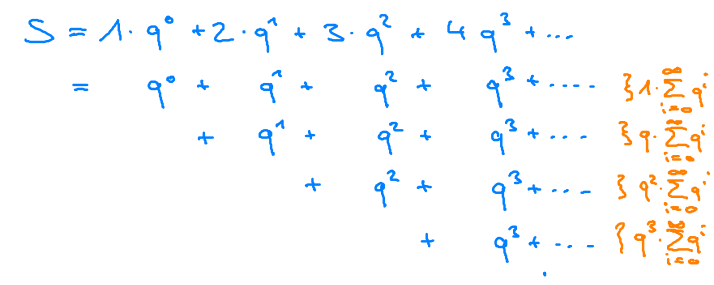
\includegraphics[width=0.7\textwidth]{SWahrscheinlichkeit.png}
\[= \bigg(\sum\limits_{i=0}^{\infty} q^i \bigg) \cdot \bigg(\sum\limits_{i=0}^{\infty} q^i \bigg) = \frac{1}{p} \cdot \frac{1}{p} = \frac{1}{p^2}\]
\[\Rightarrow E(X) = \frac{1}{p} = \frac{m}{w}\]
\textbf{Anwendung auf open addressing:}
Sondierungen $\widehat{=}$ Ziehen aus Urne\\
\[E(\# \text{ Ziehungen bis freier Platz gefunden }) = \frac{m}{m-n} = \frac{1}{1 - \frac{n}{m}} = \frac{1}{1-\alpha}\]

$\Rightarrow$ Satz $\hfill \Box$
\end{minipage}}

\begin{itemize}
\item Einfügen: im Mittel konstant (falls $\alpha < 1$ konstant)
\item Suchen: dieselbe Folge von Sondierungen wie Einfügen (sofern in der Einfügefolge nicht bereits Elemente gelöscht wurden)
\item Löschen bereitet daher Schwierigkeiten!
\end{itemize}

Daher ist open addressing meistens beschränkt auf Hashing ohne Löschen.

\subparagraph{Zusammenfassung}
Aufwand pro Operation im Mittel $O(1)$, aber im Worst Case $\Omega(n)$\\
Vergleich zu Suchbäumen: im Worst Case $O(\log n)$, mittlerer Aufwand $\Omega (\log n)$, denn:\\
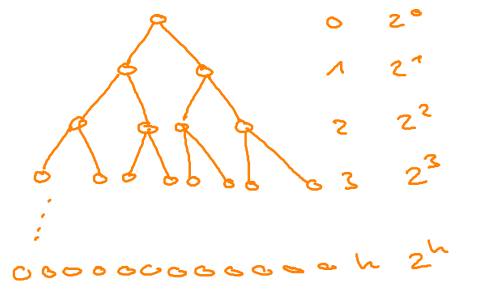
\includegraphics[width=0.8\textwidth]{./SuchbaumHoehe}\\
Beobachtung: Mindestens die Hälfte aller Knoten liegt in Tiefe $\geq \log n$\\
$ \Rightarrow $ im Average Case ist der Aufwand für Suchen $\Omega (\log n)$

\subparagraph{Universelles Hashing}
Idee: Vermeide Worst Case. Stelle bösen Gegenspieler vor, der Hashing- Verfahren und durch Auswahl spezieller Schlüssel in den Worst Case treibt. $\Rightarrow$ Randomisiere zur Laufzeit des Verfahrens, d.h. wähle eine zufällige Hash- Funktion. Diese wird dann für die gesamte Dauer des Verfahrens verwendet.
\fbox{\begin{minipage}{\textwidth}
\textbf{Definition:}\\

Eine Klasse $H$ von Hash- Funktionen heißt universell bezüglich der Größe $m$ der Hash- Tabelle, falls $\forall \,\, $ Schlüsselpaare $x, y \in U$ mit $x \neq y$ gilt:
\[| \{h \in H | h(x) = h(y) \} | \leq \frac{|H|}{m}\]
\end{minipage}} \\ 

\textbf{Idee:} Wähle $h \in H$ zufällig und gleichverteilt, dann ist die Wahrscheinlichkeit für eine Kollision von $x$ und $y \leq \frac{1}{m}$.

\textbf{Satz:} $H$ sei universell für $m, h \in H$ zufällig und gleichverteilt gewählt. Werden nun $n \leq m$ Schlüssel mit $h$ eingefügt und ist $x$ ein fester Schlüssel, so gilt: \[E (\# \text{ Kollisionen mit }x) < 1\]
\shadowbox{\begin{minipage}{0.95 \textwidth}
\textbf{Beweis:}\\

Für Schlüsselpaar $y \neq z$ sei \\
$C_{yz} = \left\{ \begin{array} {ll c l}
1; & \text{ falls } h(y) = h(z) & \text{ Wahrscheinlichkeit } & \leq \frac{1}{m}\\
0; & \text{ sonst } & \cdots & \geq \frac{m-1}{m}
\end{array}\right.$\\

$E(C_{yz}) \leq \frac{1}{m}$

Sei $C_x = \#$ Kollisionen mit $x$, d.h. $C_x = \sum\lim\limits_{y \neq x} C_{yx}$
\[E(C_x) = E(\sum\lim\limits_{y \neq x} C_{yx}) = \sum\lim\limits_{y \neq x} E(C_{yx}) \leq \frac{n-1}{m} < 1\]
$\hfill \Box$
\end{minipage}}

Angewendet auf Hashing mit chaining: Mittlere Listenlänge $ < 2$. Worst Case tritt im Erwartungswert nicht auf, Absicherung gegen bösen Gegenspieler klappt.

Zeige, dass $\exists$ universelle Klasse von Hashfunktionen für beliebiges $m$:\\

Wähle dazu zunächst Primzahl $p$ mit $p > x$ für alle $x \in U$.
Für beliebiges $a \in \mathbb{Z}_p* = \{1, ..., p-1\}$ und $b \in \mathbb{Z}_p = \{0, 1, ..., p-1\}$ sei die Hash- Funktion $h_{a,b}$ wie folgt definiert:
\[h_{a,b}(x) = ((a\cdot x + b) \mod{m})\]
Es sei $H = \{h_{a,b} | a \in \mathbb{Z}_p*, b \in \mathbb{Z}_p\}$

\textbf{Satz:} $H$ ist unversell bezüglich $m$.

\shadowbox{\begin{minipage}{0.95 \textwidth}
\textbf{Beweis:}\\

Betrachte zwei Schlüssel $x\neq y$ aus $\{0, ..., p-1\}$ und $h_{a,b} \in H$. Definiere
\[r := a \cdot x + b \mod {p}\]
\[s := a \cdot y + b \mod {p}\]

\underline{Behauptung:} $x\neq y \Rightarrow r \neq s$\\
\underline{Beweis:} Annahme: $r = s$
\[ \Rightarrow a \cdot x + b \equiv a \cdot y + b \mod{p}\]
\[\overset{a \in \mathbb{Z}_p*}{\Rightarrow} x \equiv y \mod{p} \Rightarrow x = y \text{\textbf{ Widerspruch!}} \hfill \blacksquare\]

\underline{Behauptung:} $a$ und $b$ sind eindeutig durch $x, y, r, s$ bestimmt.\\
\underline{Beweis:} Aus der Definition folgt:
\[(r-s) \equiv a \cot \underbrace{(x-y)}_{\in \mathbb{Z}_p*} \mod{p}\]
\[\Rightarrow a = (x-y)^{-1} \cdot (r-s) \in \mathbb{Z}_p\]

\[r = a\cdot x + b \Rightarrow b = r-(x-y)^{-1} \cdot (r-s) \cdot x \hfill \blacksquare\]

Es gibt $(p-1) \cdot p$ Paare $r,s \in \{0, ..., p-1\}$ mit $r \neq s$.\\
$\Rightarrow$ Es gibt Bijektion zwischen möglichen Paaren $(a,b)$ und $(r,s)$.\\
$\Rightarrow$ Wählt man eine zufällige Hash- Funktion aus $H$, also ein zufälliges Paar $(a, b)$, dann erhält man ein zufälliges Paar $(r, s)$.

Es gilt:
\[Pr (h_{a,b} (x) = h_{a,b}(y)) = Pr (r \equiv s \mod{m})\]

Für festes $r$ gibt es $\leq \lceil \frac{p}{m} \rceil -1$ mögliche $s \neq r$ mit $r \equiv s \mod{m}$.

Es gilt:
\[\lceil \frac{p}{m} \rceil -1 \leq \frac{p+m-1}{m} -1 = \frac{p-1}{m}\]
Daraus folgt: Die Wahrscheinlichkeit dafür, dass ein zufälliges $s \in \{0, ..., p-1\} \setminus \{r\}$ zu einer Kollision führt ist $\leq \frac{1}{m}$.

$\Rightarrow H$ ist universell bezüglich $m$.
$\hfill \Box$
\end{minipage}}

\newpage
\paragraph{Perfektes Hashing:}
\begin{itemize}
\item Nehme an, dass Schlüsselmenge statisch und a priori bekannt ist, z.B.
\begin{itemize}
\item reservierte Worte in Java (Compiler verwendet Hashing)
\item Namen aller Dateien auf DVD
\end{itemize}
\item Ziel: Verbessere den Worst- Case- Aufwand für die Suche (im Mittel Aufwand $O(1)$)
\item Ein Hashing- Verfahren heißt perfekt, $\Leftrightarrow$ Worst- Case- Aufwand für das Suchen ist $O(1)$.
\end{itemize}

\subparagraph{Umsetzung}

\begin{itemize}
\item Mithilfe eines zweistufigen Verfahrens:\\
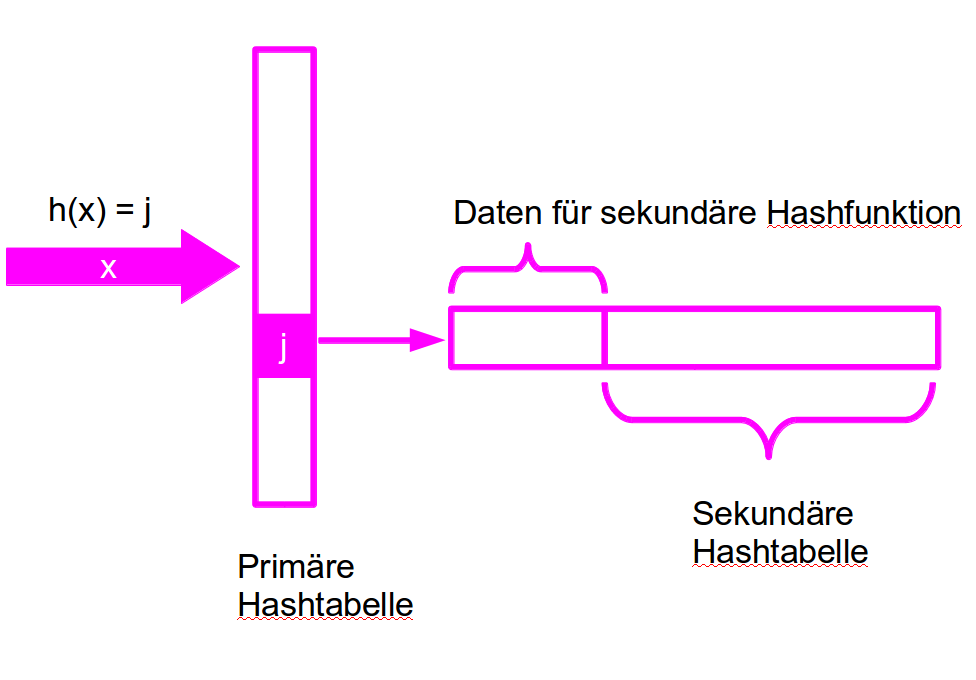
\includegraphics[width=0.6\textwidth]{PerfektesHashing.png}
\item Daten für sekundäre Hashfunktion $h_j$ und Länge der sekundären Hash- Tabelle werden in der sekundären Hash- Tabelle zu Beginn gespeichert.
\item Die sekundäre Hash- Tabelle hat die Länge $m_j$, dieses hängt ab von\\ $h_j := \#$ Schlüssel mit $h(x) = j$, nämlich $m_j = h_j^2$
\item Bemerkung: $h_j$ kann man vorab (nach Wahl von $h$) bestimmen, da alle Schlüssel bekannt.
\item Die Primäre Hashfunktion $h$ und sekundäre Hashfunktionen $h_j, j = 1, ..., m$ sind aus universeller Klasse gewählt:
\[h(x) = ((a\cdot x + b) \mod{p} )\mod{m}\]
\[h_j(x) = ((a_j \cdot x + b_j) \mod{p}) \mod{m_j}\]
\begin{itemize}
\item $h(x) \in H_{p, m}$
\item $h_j(x) \in H_{p, m_j}$
\item $p$ Primzahl $> x \quad \forall \quad $ Schlüssel $x$
\item $m$ Länge primärer Hashtabelle
\item $m_j = h_j^2$
\end{itemize}
\item Spezialfall: Falls $h_j = 1$, wähle $a_j = b_j = 0, m_j = h_j^2 = 1$
\item Zwei mögliche Probleme
\begin{itemize}
\item[A] Wie stellt man sicher, dass beim sekundären Hashing keine Kollision auftritt?
\item[B] Kann der benötigte Speicherplatz sinnvoll beschränkt werden?
\end{itemize} 
\end{itemize}


Zu A: \textbf{Satz:} Eigenschaft der sekundären Hashfunktion mit $n =  n_j, m = m_j$\\

$n$ Schlüssel: werden mit zufällig gewählter Hashfunktion $h \in H_{p,m}$ in Hashtabelle der Länge $m = n^2$ gespeichert. Dann ist die Wahrscheinlichkeit, dass eine Kollision auftritt, klein, d.h. $< \frac{1}{2}$.\\

Das heißt, dass bei wiederholter zufälliger Wahl von $h \in H_{p, m}$ \textbf{mit großer Wahrscheinlichkeit} \textit{nach wenigen Wiederholungen} eine kollisionsfreie Hashfunktion gefunden wird.

\shadowbox{\begin{minipage}{0.95 \textwidth}
\textbf{Beweis:}\\
$\exists$ insgesamt $\bigg(\begin{array}{c} n \\ 2 \end{array} \bigg)$ mögliche Kollisionen.

$H_{p, m}$ ist universell $\Rightarrow x \neq y$ kollidieren mit Wahrscheinlichkeit $\leq \frac{1}{m}$.

Sei $X = \# $ Kollisionen, dann gilt:
\[E(X) = E (\sum\limits_{x\neq y} C_{x, y}) = \sum\limits_{x \neq y} E (C_{x, y}) \leq \bigg(\begin{array}{c} n \\ 2 \end{array} \bigg) \cdot \frac{1}{m} = \frac{n(n-1)}{2} \cdot \frac{1}{n^2} < \frac{1}{2}\]
\centering
\framebox {\begin{minipage} {0.9\textwidth}
\underline{Markov'sche Ungleichung:}

Für eine Zufallsgröße $X \geq 0$ und $t > 0$ gilt:
\[P_r (X \geq t) \leq \frac{E(X)}{t}\]
\end{minipage}}
\flushleft

In unserem Fall:

\[P_r(X \geq 1) \leq \frac{E(X)}{1} < \frac{1}{2}\]
Problem A gelöst: $\hfill \Box$
\end{minipage}}

\textbf{Satz:} Die Wahrscheinlichkeit für das Auftreten eines Konfliktes in einer sekundären Hashtabelle ist bei zufälliger Wahl von $a_j$ und $b_j$ kleiner als $\frac{1}{2}$.\\
$\Rightarrow \exists \quad a_j, b_j$ mit konfliktfreier sekundärer Hashfunktion.\\\\

\textbf{Satz:} Die Wahrscheinlichkeit für das Auftreten eines Konfliktes in einer sekundären Hashtabelle ist bei zufälliger Wahl von $a_j$ und $b_j$ kleiner als $\frac{1}{2}$.\\
$\Rightarrow \exists \quad a_j, b_j$ mit konfliktfreier sekundärer Hashfunktion.\\\\

Zu B: \textbf{Satz:} $n$ Schlüssel werden mit zufälliger Hashfunktion $h \in H_{p, m}$ in eine Hashtabelle der Größe $m = n$ gespeichert.
Dann gilt: $E\bigg(\sum\limits_{j = 0}^{m-1}n_j^2\bigg) < 2 \cdot n$ wobei $m_j := |\{x | h(x) = j\}$\\

\shadowbox{\begin{minipage}{0.95 \textwidth}
\textbf{Beweis:}\\
Für $a \in \mathbb{N}$ gilt: $a^2 = a+2 \bigg( \begin{array}{c}
a \\ 2 \end{array} \bigg)$
Unter Betrachtung der Linearität des Erwartungswertes gilt:
\[E \bigg(\sum\limits_{j = 0}^{m-1} n_j^2\bigg) = E\bigg(\sum\limits_{j=0}^{m-1} \bigg(n_j + 2 \bigg( \begin{array}{c}
n_j \\ 2 \end{array} \bigg) \bigg)\bigg) =\]
\[ E\bigg(\underbrace{\sum\limits_{j=0}^{m-1} n_j}_{n}\bigg) + 2 \cdot E\bigg(\sum\limits_{j=0}^{m-1} \begin{array}{c}
n_j \\ 2 \end{array} \bigg) = \]
\[n +  2 \cdot \underbrace{E\bigg(\sum\limits_{j=0}^{m-1} \underbrace{\begin{array}{c}
n_j \\ 2 \end{array} \bigg)}_{\# \, Kollisionen \, an \, Stelle \, j}}_{\# \, Kollisionen , insgesamt} \leq n + 2 \cdot \bigg(\begin{array}{c}
n \\ 2 \end{array} \bigg) \cdot \frac{1}{m}\]
\[= n + (n-1) = n+n-1 = 2 n - 1 < 2n\]
 $\hfill \Box$
\end{minipage}}

\textbf{Korollar:} Für das zweistufige Hashverfahren mit primärer Länge $m = n$ und sekundärer Länge $m_j = n_j^2$ gilt: Der erwartete Speicherbedarf ist linear in $n$, d.h. $O(n)$.

\textbf{Satz:} Für das zweistufige Hash- Verfahren gilt:
\[P_r (\text{ Speicherbedarf für sekundäre Hashtabelle } \geq 4n) < \frac{1}{2}\]
$\Rightarrow$ Probiere so lange zufällige primäre Hash- Funktion aus, bis Speicher $ < 4n$ (Beweis: Markov'sche Ungleichung) $\hfill \Box$\\
$\Rightarrow$ Durch wiederholtes Ziehen einer zufälligen primären Hash- Funktion $h$ kann man garantieren, dass der Speicherbedarf $\leq 4n$ ist.

\newpage
\section{Berechenbarkeit und Komplexität}
Grundfrage dieses Kapitels: Welche Probleme lassen sich mit Computern lösen? Welche Probleme lassen sich effizient lösen? Dazu müssen aber diese beiden Fragen geklärt sein:
\begin{itemize}
\item Was ist ein Computer?
\item Was ist ein Problem?
\end{itemize}

\subsection{Computer}
\subsubsection{Grundidee}
\begin{center}
\Ovalbox{\begin{minipage}{0.6\textwidth}
\centering
$\underset{\in \Sigma^*}{\text{Eingabe}} \rightarrow \text{Computer} \rightarrow \underset{\in \Sigma^*}{\text{Ausgabe}}$
\end{minipage}}
\end{center}
$\Sigma$ - endliches Alphabet, z.B. $\{0, 1\}$\\
$\Sigma^* := \bigcup\limits_{i = 1}^{\infty} \Sigma^i$ - Menge der Strings endlicher Länge über $\Sigma$\\
\subsubsection{Turing- Maschine}$ $\\
\includegraphics[width=\textwidth]{TuringMaschine.png}
\begin{itemize}
\item[\textbf{Bandalphabet}] $\Gamma = \Sigma \cup \{B\} \cup \{...\}$, wie Alphabet $\Sigma$ endlich.
\item[\textbf{Programm}] $\delta : Q \times \Gamma \rightarrow Q \times \Gamma \times \{R, L, N\}$:
Eine eindeutige Handlungsanweisung, die ausgehend vom aktuellen Zustand der Maschine und dem gelesenen Zeichen der Maschine einen neuen Zustand, ein zu schreibendes Zeichen und eine Bewegungsanweisung vorgibt.
Bewegungsanweisung kann ein Feld nach rechts oder links oder auch stehen bleiben bedeuten.
\item[\textbf{Deterministische Turing- Maschine (DTM)}] Jeder Schritt wird nur durch Eingabe und Programm vorherbestimmt, es gibt keine zufälligen Schritte.
\item[\textbf{Nicht- Terministische Turing- Maschine}] Hier können Schritte zufallsgesteuert ablaufen, man kann \glqq auf einen Zufallsgenerator zugreifen\grqq.
\item[\textbf{Konfiguration einer DTM}] Besteht aus $\alpha, q, \beta$ mit $\alpha, \beta \in \Sigma^*, q \in Q$. $\alpha$  die Symbole auf dem Band links vom Kopf, $\beta$ die restlichen, beginnend unter dem Kopf bis zum rechten Ende des Bereichs. $q$ ist der Zustand der DTM.
\item[\textbf{Direkte Nachfolgekonfiguration}] von $\alpha, q, \beta$ ist $\alpha', q', \beta'$, falls man in einem Schritt von $\alpha, q, \beta$ zu $\alpha', q', \beta$ kommt. $\alpha, q, \beta \vdash \alpha', q', \beta'$
\item[\textbf{Nachfolgekonfiguration}] von $\alpha, q, \beta$ ist $\alpha'', q'', \beta''$, falls man in endlich vielen Schritten von $\alpha, q, \beta$ zu $\alpha'', q'', \beta''$ kommt. $\alpha, q, \beta \vdash^* \alpha'', q'', \beta''$
\end{itemize}

\paragraph{Mehrspur- Turing- Maschinen}
Modelliere $k$ Spuren durch Ersetzen von $\Gamma$ durch $\Gamma^k$.
\paragraph{Mehrband- Turing- Maschinen}
Allgemein: $k$ Bänder, $\delta: Q \times \Gamma^k \rightarrow Q \times \Gamma^k \times \{L, R, N\}^k$

\textbf{Satz:} Eine $k$- Band- TM $M$, die mit Rechenzeit $t(n)$ und Platz $s(n)$ auskommt, kann von einer TM $M'$ mit Rechenzeit $O(t(n)^2)$ und Platz $O(s(n))$ emuliert werden.\\\\
\shadowbox{\begin{minipage}{0.95 \textwidth}
\textbf{Beweisidee:}\\
Benutze Mehr- Spur- TM $M'$ mit $2k+1$ Spuren
\begin{itemize}
\item[$\rightarrow$] Fahre Band ab, markiere einzelne Kopf-Positionen (Sprung)
%%%Hier Recherche!!!%%%
\item[$\rightarrow$] Fahre dann nochmal ab und führe Mehrband- Programm aus
\end{itemize}
Größe des Bereichs $\in O(t(n))$
\end{minipage}}
 
 \newpage
\paragraph{Universelle Turing- Maschine}
Betrachte Turing- Maschine $M$ mit (o.B.d.A.):\\
$\Sigma = \{0, 1\}$ und $\Gamma = \{0, 1, B\} = \{x_1, x_2, x_3\}$\\
$D_1 = L; D_2 = R; D_3 = N$\\
$Q = \{q_1, q_2, ..., q_t\}; F = \{q_2\}$
Kodiere Programm $\delta$ von $M$ wie folgt:

$\delta (q_i, x_j) = (q_n, x_l, D_M) \quad \quad z = 1, ..., s$
\[0^i10^j10^k10^l10^m = Code(z)\]

\subparagraph{Definition Gödelnummer:} Die Gödel- Nummer der Turing- Maschine $M$ ist: 

\[111Code(1)11Code(2)11...11Code(s)111 =: <M>\] 

\subparagraph{Definition Universelle Turing- Maschine:} Eine universelle Turing- Maschine $U$ erwartet als EIngabe eine Gödelnummer und ein Wort $W$ als Paar: $(<M>, W)$, wobei $M$ eine TM und $W \in \{0, 1\}^*$. $U$ simuliert $M$ auf der Eingabe $W$.

\subparagraph{Realisierung von $U$ als Drei- Band- TM}
\begin{itemize}
\item[1] Teste Eingabe auf Korrektheit: $i, k \geq 1; j, l, m \in \{1, 2, 3\}$

Keine zwei Codes dürfen mit demselben Präfix $0^i10^j$

...
\item[2] Kopiere $<M>$ auf Band 2 und überschreibe sie auf Band 1 mit Leerzeichen
\item[3] Schreibe Zustand $q_i$ von $M$ auf Band 3, kodiert als $0^i$.
\item[4] In jedem Schritt:
\begin{itemize}
\item Lese $x_j$ auf Band 1, suche auf Band 2 den zugehörigen String $110^i10^j1...$, wobei $0^i$ auf Band 3 steht.
\item Akzeptiere, falls $i = 2$

Andernfalls: 
\begin{itemize}
\item[] Lese $0^k10^l10^m11$ auf Band 2 
\item[] Schreibe $0^k$ auf Band 3
\item[] Schreibe $x_l$ auf Band 1
\item[] Bewege Kopf von Band 1 in Richtung $D_m$
\end{itemize}
\end{itemize}
\end{itemize}

\subparagraph{Beobachtung}
Für festes $M$ ist die Rechenzeit von $U$ auf der Eingabe $<M>, W$ nur um einen konstanten Faktor größer, als die Rechenzeit von $M$ auf $W$.

\subparagraph{Church'sche These}
\begin{itemize}
\item Die durch die formale Definition der Turing- Maschine erfasste Klasse berechenbarer Funktionen stimmt überein mit der Klasse der intuitiv berechenbaren Funktionen.
\item Die Turing- Maschine erfasst die Rechenzeit bis auf polynomielle Faktoren richtig.
\end{itemize}
\subsection{Problem}
Eine Relation $R$ auf $\Sigma^* \times \Sigma^*$ mit $(x, y) \in \mathbb{R} \Leftrightarrow y \in \Sigma^*$ ist zulässige Ausgabe zur Eingabe $x \in \Sigma^*$
\subsubsection{Spezialfall Funktion} 
\[f : \Sigma^* \rightarrow \Sigma^*\]
Gegeben: $x \in \Sigma^*$\\
Gesucht: $y := f(x) \in \Sigma^*$

\subsubsection{Entscheidungsprobleme}
Ein Spezialfall der Funktionen.
\[f : \Sigma^* \rightarrow \{0, 1\}\]
Gegeben: $x \in \Sigma^*$
Entscheide, ob $f(x) = 1$.

\paragraph{zugehörige Sprache} $L := f^{-1} (1) \subseteq \Sigma^*$

\subsubsection{Es gibt unlösbare Probleme}
Computerprogramme $\subseteq \{0, 1\}^*$
Es gibt \glqq nur\grqq abzählbar unendlich viele Computerprogramme.

Probleme $\supseteq \{0, 1\}^{(\{0, 1\}^*)} \qquad \widetilde{=} \,\, \mathbb{R} \Rightarrow$ Fast alle Probleme sind unlösbar.

\newpage
\subsection{Berechenbarkeit}
\paragraph{Definitionen}
DTM = deterministische Turing- Maschine
\begin{itemize}
\item[1]$f: \Sigma^* \rightarrow \Sigma^*$ heißt total rekursiv oder berechenbar, falls $\exists$ DTM, die zur Eingabe $x \in \Sigma^*$ die Ausgabe $f(x) \in \Sigma^*$ erzeugt.
\item[2]$f : \mathbb{N}^* \rightarrow \mathbb{N}$ heißt total rekursiv, falls $\exists$ DTM, die zur Eingabe \\
$bin(i_1) \# bin(i_2) \# ... \# bin(i_k)$ die Ausgabe $bin(m)$ erzeugt,\\
wobei $m = f(i_1, i_2, ..., i_k)$.
\item[3] Eine Sprache $L \subseteq \Sigma^*$ heißt rekursiv (entscheidbar), wenn $\exists$ DTM, die auf alle Eingaben $\in \Sigma^*$ stoppt und die Eingabe $w \in \Sigma^*$ genau dann akzeptiert, wenn $w \in L$.
\item[4] Eine Sprache $L \subseteq \Sigma^*$ heißt rekursiv aufzählbar (semi- entscheidbar), wenn $\exists$ DTM, die genau die Eingaben aus $L$ akzeptiert. (Stopp bei Eingaben $\in \Sigma^* \setminus \{L\}$ nicht gefordert.)

\end{itemize}

\subsubsection{Unentscheidbare Probleme}
\paragraph{Die Diagonalsprache}
\subparagraph{Definition Kanonische Ordnung} Für $w, w' \in \Sigma^*$ schreibe $w \leq w'$, falls $w$ kürzer ist als $w'$ oder beide gleich lang sind und $w$ lexikographisch kleiner ist als $w'$. Definiert totale Ordnung auf $\Sigma^*$.
\subparagraph{Definition Diagonalsprache} Sei $M_i$ die DTM, deren Gödelnummer an $i$- ter Stelle in der Liste aller Gödelnummern steht, $w_i$ das Wort aus $\Sigma^*$, das an  $i$- ter Stelle in der kanonischen Ordnung von $\Sigma*$ steht. Die Diagonalsprache ist definiert als
\[D := \{w_i | M_i \text{ akzeptiert } w_i \text{ nicht }\}\]
\subparagraph{Satz} $D$ ist nicht rekursiv.\\\\
%
\shadowbox{\begin{minipage}{0.95 \textwidth}
\subparagraph{Beweis}
Angenommen, $\exists$ DTM, die $D$ entscheidet.

Es gilt: $M = M_j$ für ein $j \in \mathbb{Z} > 0$.\\

Frage: Was liefert $M_j$ bei Eingabe $w_j$?\\

\underline{1. Fall} $w_j \in D \Rightarrow M_j$ akzeptiert $w_j$\\
aber nach Definition von $D$ akzeptiert $M_j w_j$ nicht. $\Rightarrow$ \textbf{Widerspruch!}$\hfill \blacksquare$\\
%
\underline{2. Fall} $w_j \notin D \Rightarrow M_j$ akzeptiert $w_j$ nicht\\
aber nach Definition von $D$ akzeptiert $M_j w_j$. $\Rightarrow$ \textbf{Widerspruch!} $\hfill \blacksquare$\\
Es gibt keine DTM, die $D$ entscheidet. $\hfill \square$
\end{minipage}}
\subparagraph{Korollar} $\bar{D} := \Sigma^* \setminus D$ ist auch nicht rekursiv.\\
%
\shadowbox{\begin{minipage}{0.95 \textwidth}
\textbf{Beweis}
Eine Sprache $L$ ist rekursiv $\Leftrightarrow$ ihr Komplement ist rekursiv.\\
(Vertausche akzeptierende und nicht akzeptierende Endzustände der zugehörigen DTM.) $\hfill \square$
\end{minipage}}

\paragraph{Das Halteproblem}
\subparagraph{Definition Halteproblem}
\[H := \{<M>w \,\,|\,\, M \text{ hält auf }w\}\]
\subparagraph{Satz} $H$ ist nicht rekursiv.\\\\
%
\shadowbox{\begin{minipage}{0.95 \textwidth}
\subparagraph{Beweis}
Angenommen, $M$ ist DTM, die $H$ entscheidet. Mit $M$ konstruiere DTM $M'$, die das Komplement der Diagonalsprache entscheidet.\\
Es sei $w \in \Sigma^*$, entscheide ob $w \in \bar{D}$. 
\begin{itemize}
\item Berechne $i$ mit $w = w_i$
\item Berechne $<M_i>$
\item Wende $M$ an auf $<M_i>w$
\begin{itemize}
\item Falls $<M_i>w \notin H$, so ist $w \notin \bar{D}$.
\item Falls $<M_i>w \in H$ simuliere $M_i$ auf Eingabe $w$ (mit Hilfe der universellen DTM). $M_i$ akzeptiert $w_i \Leftrightarrow w_i \in \bar{D}$. 
\end{itemize}
\end{itemize}
Damit ließe ich $D$ entscheiden. $\Rightarrow$ \textbf{Widerspruch!} $\hfill \square$
\end{minipage}}

\paragraph{Das spezielle Halteproblem}
\subparagraph{Definition spezielles Halteproblem}
Das spezielle Halteproblem $H_\epsilon$ ist definiert durch
\[H_\epsilon = \{<M> \,\, | \,\, M \text{ hält auf } \epsilon \text{ an } \} \]
Dabei ist $\epsilon$ das leere Wort.
\subparagraph{Satz} $H_\epsilon$ ist nicht rekursiv.\\\\
\shadowbox{\begin{minipage}{0.95 \textwidth}
\subparagraph{Beweis}
Annahme: DTM $M'$ entscheidet $H_\epsilon$. Konstruiere daraus TM $M''$, die $H$ entscheidet:
\begin{itemize}
\item $M''$ berechnet auf Eingabe $<M>w$ zunächst $<M_w''>$, die Folgendes leistet:
\subitem Schreibe $w$ auf das Band und simuliere $M$ auf $w$.
\item $M''$ simuliert $M'$ auf $<M_w''>$
\item[$\rightarrow$] Dann gilt: $M''$ akzeptiert $<M>w \Leftrightarrow M_w''$ hält auf $\epsilon$ an $\Leftrightarrow M$ hält auf $w$ an. $\hfill \square$
\end{itemize}
\end{minipage}}
\subparagraph{Korollar} $\bar{H_\epsilon}$ ist nicht rekursiv.

\paragraph{Die universelle Sprache}
\subparagraph{Definition universelle Sprache}
\[U = \{<M>w \,\,|\,\,M \text{ akzeptiert } w\}\]
\subparagraph{Satz} $U$ ist nicht rekursiv.\\\\
\shadowbox{\begin{minipage}{0.95 \textwidth}
\subparagraph{Beweis}
Andernfalls $\exists$ DTM $M$, die $\bar{D}$ entscheidet.

Gegeben: $w \in \Sigma^*$, ist $w \in \bar{D}$?

Berechne $i$, sodass $w = w_i$ und $<M_i>$. Entscheide, ob $<M_i>w_i \in U$.
\end{minipage}}

\subparagraph{Satz} $U$ ist rekursiv aufzählbar (semi- entscheidbar).\\\\
\shadowbox{\begin{minipage}{0.95 \textwidth}
\subparagraph{Beweis}
Wende die universelle DTM an auf $<M>w$. Falls $M w$ akzeptiert geschieht das nach endlich vielen Schritten $\rightarrow$ Ausgabe nach endlich vielen Schritten.
\end{minipage}}

\paragraph{Satz von Rice}
\subparagraph{Definition zur Berechenbarkeit} Sei $Q \subseteq \Sigma^*, f : Q \rightarrow \Sigma^*$.

$f$ heißt berechenbar, wenn $\exists$ DTM, die auf die Eingabe $x \in Q$ die Ausgabe $f(x)$ liefert und für Eingabe $x \notin Q$ nicht anhält oder nicht akzeptiert.

\textbf{Spezielles Beispiel:}
$Q=\emptyset$(leere Menge)\\
$U:\emptyset \rightarrow \Sigma^*$ ist berechenbar.

Zugehörige DTM: Gehe im ersten Schritt in nicht- akzeptierenden Endzustand.

\subparagraph{Satz von Rice} Sei $R$ die Menge aller berechenbaren Funktionen und $\emptyset \neq S \subsetneqq R$ eine nichttriviale Teilmenge von $R$. Dann ist die Sprache $L(S) := \{<M> | M \text{ berechnet Funktion aus } S\}$ nicht rekursiv.

Das heißt: Ein Computer kann keinerlei bedeutende Aussagen über einen gegebenen Algorithmus treffen.

\subparagraph{Beweis} Erfolgt per Widerspruch:\\
\textbf{Annahme:} $M_S$ entscheidet $L(S)$. Konstruiere daraus eine DTM $M'$, die $\bar{H_\epsilon}$ entscheidet.\\

Betrachte im Folgenden die spezielle Funktion $U \in R$ mit
\[U: \emptyset \rightarrow \Sigma^*\]
%
Nehme o.B.d.A. an, dass $u \in S$. Andernfalls ersetze $S$ durch $R \setminus S$ und beachte, dass $L(R\setminus S = \overline{L(S)})$.\\
%
Weiter sei $f \in R\setminus S$ und $M_f$ eine DTM, die $F$ berechnet.\\\\
%
Die DTM $M'$ arbeitet wie folgt (bei Eingabe $<M>$):
\begin{itemize}
\item[1] Berechne Gödelnummer $<M''>$ der DTM $M''$, die auf Eingabe $x$ Folgendes tut:
\begin{itemize}
\item $M''$ simuliert $M$ auf Eingabe $\epsilon$
\item Falls $M$ auf $\epsilon$ anhält, so simuliert $M''$ die DTM $M_f$ auf $x$.
\end{itemize}
\item[2] Simuliere DTM $M_S$ auf $<M''>$.
\end{itemize}

\textbf{Dann gilt:}
\begin{itemize}
\item[1. Fall:] $M$ hält auf $\epsilon$ nicht an
\begin{itemize}
\item[$\Rightarrow$] $M''$ berechnet $U \in S$
\item[$\Rightarrow$] $M_S$ akzeptiert $<M''>$
\item[$\Rightarrow$] $M'$ akzeptiert $<M>$
\end{itemize}
\item[2. Fall:] $M$ hält auf $\epsilon$ an
\begin{itemize}
\item[$\Rightarrow$] $M''$ berechnet $f \in R \setminus S$
\item[$\Rightarrow$] $M_S$ akzeptiert $<M''>$ nicht
\item[$\Rightarrow$] $M'$ akzeptiert $<M>$ nicht.
\end{itemize}
\end{itemize}
Folglich entscheidet $M'$ die Sprache $\overline{H_\epsilon}$. $\Rightarrow$ \textbf{Widerspruch!} $\hfill \square$

\newpage
\subsection{Der Gödel'sche Unvollständigkeitssatz}
\subsubsection{Satz von Church}
\paragraph{Definition Sprache der wahren Sätze}
Für eine fest vorgegebene Menge an Relationen $\{R;1, ..., R_k\}$ sei $L$ die Sprache der wahren Sätze:
$L = \{Q_1x_1 ... Q_lx_l \Phi = S\,\,|\,\, S \text{ ist wahrer Satz } \}$
\paragraph{Satz von Church} $L$ ist nicht rekursiv, falls unter den Relationen $R_1, ..., R_k$ die Additionsrelation und die Multiplikationsrelation ist.

\subparagraph{Beispiel} Es ist nicht entscheidbar, ob ein Polynom über mehreren Variablen eine ganzzahlige Nullstelle besitzt.

\subsubsection{Annahmen über Beweise}
Der Gödelsche Unvollständigkeitssatz beruht auf folgenden Annahmen über \glqq Beweise\grqq von Sätzen:
\begin{itemize}
\item[1] Ein Beweis $\Pi$ eines Satzes $S$ kann von einer DTM überprüft werden, d.h.
\[\{S\Pi \,\, | \,\, \Pi \text{ ist Beweis von }S \}\]
ist rekursiv.
\item[2] Ist $\Pi$ ein Beweis von $S$, so ist $S$ wahr.
\end{itemize}
Unter diesen Annahmen gilt:
\paragraph{Satz} Die Sprache $L'$ aller beweisbaren Sätze ist rekursiv aufzählbar.
\[L' := \{S\,\,|\,\,\exists \text{ Beweis } \Pi \text{ für }S\}\]
\paragraph{Beweis} Zu einem gegebenen Satz überprüft man alle möglichen \glqq Beweis\grqq der Reihe nach, nach aufsteigender Länge mithilfe der DTM aus Annahme 1.

Gibt es also einen gültigen Beweis für $S$, so wird dieser in endlicher Zeit gefunden.

\subsubsection{Gödel'scher Unvolsständigkeitssatz}
\paragraph{Satz} Es sei $L$ die Sprache der wahren Sätze, die mittels Additions- und Multiplikationsrelation formuliert werden können.

Dann gibt es Sätze in $L$, die nicht beweisbar sind.

\paragraph{Beweis} Durch Widerspruch\\
Nehme an, dass $L = L'$. Betrachte gegebenen Satz $S$. Dann ist entweder $S$ oder seine Negierung wahr.

Wende die DTM aus dem viorigen Beweis parallel an auf $S$ und die Negierung von $S$.

Da einer von beiden Sätzen wahr ist, gibt es (unter der Widerspruchsannahme $L = L'$) einen Beweis für einen von beiden, der in endlicher Zeit gefunden wird.\\
$\Rightarrow L$ ist rekursiv.\\
$\Rightarrow$ Widerspruch zum Satz von Church $\hfill \square$

\subsection{Komplexitätsklasse P und NP- Vollständigkeit}
\subsubsection{Definitionen}
\subparagraph{Definition} Sei $M$ DTM auf Eingabealphabet $\Sigma$. Die worst- case- Rechenzeit $t_M(n)$ ist die maximale Anzahl Rechenschritte, die $M$ auf einer Eingabe aus $\Sigma^n$ durchführt.
\subparagraph{Definition} $P$ ist  die Klasse der Sprachen $L$ (Entscheidungsprobleme), für die $\exists $ DTM $M$, die $L$ entscheidet und
\[t_M(n) \leq p(n)\]
für eine Polynomfunktion $p$.
\subparagraph{Definition} Eine Sprache (ein Problem) in $P$ heißt \textbf{effizient entscheidbar}. Der zugehörige Algorithmus (DTM) wird dann \textbf{effizient} genannt.

\subsubsection{Ist ein Problem effizient lösbar?}
Wie zeigt man, dass ein Problem nicht effizient lösbar ist?
\begin{itemize}
\item[1] Zeige, dass das Problem nicht entscheidbar ist.
\item[2] Zeige, dass die erwartete Ausgabe nicht polynomial in der Eingabegröße beschränkt ist. 

(Normalerweise ist so ein Problem dann falsch gestellt.)
\item[3] Direkte Beweise (nur in seltenen Fällen bekannt, z.B. Pressburger Arithmetik)
\end{itemize}

Keiner dieser drei Ansätze ist praktisch zufriedenstellend.

\newpage
\paragraph{Das Cliquenproblem}
\subparagraph{Definition}
Es sei $G = (V, E)$ ein ungerichteter Graph. Dann bildet $V' \subseteq V$ eine Clique, wenn $\forall$ Paare $u, v \in V'$ mit $u \neq v$ eine Kante zwischen $u$ und $v$ existiert.

\subparagraph{Varianten} $ $\\
\textbf{1. Variante:} Gegeben $G = (V, E), k \in \mathbb{N}$.\\
Gibt es eine Clique $V' \subseteq V$ mit $|V'| = k$?\\ (Entscheidungsproblem)\\\\
\textbf{2. Variante} Gegeben $G = (V, E)$\\
Berechne das größte $k \in \mathbb{N}$, sodass $G$ eine Clique der Größe $K$ besitzt.\\
(Optimierungsproblem)\\\\
\textbf{3. Variante} Gegeben $G = (V, E)$\\
Finde $V' \subseteq V$ in $G$, sodass $V'$ eine maximale Clique ist, d.h. $|V'|$ maximal.\\
(Optimierungsproblem) 

\subparagraph{Satz} Gibt es für eine der 3 Varianten des Cliquenproblems einen effizienten Algorithmus, dann auch für die anderen beiden.

\textbf{Bemerkung:} Beachte, dass $\exists$ unterschiedliche Arten, einen Graphen zu codieren (z.B., Adjazenzmatrix, Adjazenzlisten, ...). Diese unterscheiden sich in der Größe jedoch nur um polynomielle Faktoren.

\subparagraph{Beweis}
\begin{itemize}
\item Kann man Variante 3 effizient lösen, dann auch Variante 1 und 2.
\item Ein effizienter Algorithmus für Variante 2 löst auch Variante 1 effizient.
\item Zeige noch, dass ein effizienter Algorithmus für Variante 1 auch Variante 3 effizient löst.
\end{itemize}

Gegeben effiziente Unterroutine für Variante 1, konstruiere effizienten Algorithmus für Variante 3:
\begin{itemize}
\item[1] For $k = 1$ to $n$: Rufe Unterroutine auf für $G=(V, E)$ und $k$.

Bestimme dabei $max k = k^*$, für das die Antwort ja ist.
\item[2] For all $v \in V$: Rufe Unterroutine auf für den Graphen $G'$, der durch Löschen von $v$ entsteht, und für $k^*$.

Falls \glqq ja\grqq, dann lösche $v$ aus $G$.
\end{itemize}

Nach Schritt 2 bleibt von $G$ nur noch eine Clique der Größe $k^*$ übrig. $\hfill \square$

Diese Beobachtung gilt im Wesentlichen für alle Optimierungsprobleme. Daher genügt es, die Komplexität der zugehörigen Entscheidungsprobleme zu studieren.

\subsubsection{Komplexitätsklasse NP}
\subsubsection{Nichtdeterministische Turing- Maschine}
\textbf{Beobachtung:} Es scheint algorithmisch schwer zu sein, das Cliquenproblem zu lösen, d.h. es ist kein effizienter Algorithmus bekannt.\\
\textbf{Aber:} Bekommt man eine Lösung (Clique) genannt, so kann man leicht überprüfen, ob dies eine zulässige Lösung ist.
\paragraph{Definition Nichtdeterministische TM} Eine NTM ist wie eine DTM definiert, mit dem einzigen Unterschied, dass die Funktion 
\[\delta : Q \times \Gamma \rightarrow (Q \times \Gamma \times \{L, R, N\})\]
durch eine Relastion $\delta$ auf \[(Q \times \Gamma) \times (Q \times \Gamma \times \{L, R, N\})\] ersetzt wird.

Ist die NTM im Zustand $q \in Q$ und liest $a \in \Gamma$, so kann sie sich in den Zustand $q' \in Q$ begeben, das Zeichen $a' \in \Gamma$ schreiben und den Kopf in Richtung $d \in \{L, R, N\}$ bewegen, falls
\[((q, a), (q', a', d)) \in \delta\]

Die NTM hat daher unter Umständen mehrere Möglichkeiten in einem Rechenschritt. Daher ergeben sich für eine Eingabe mehrere Rechenwege und zugehörige Ausgaben.
\subparagraph{Definition} Eine NTM $M$ akzeptiert die Eingabe $w$, falls es mindestens einen Rechenweg gibt, der zu einem akzeptierenden Endzustand führt.
\[L(M) := \{w \in \Sigma* \,\, | \,\, M \text{ akzeptiert } w\}\]
\subparagraph{Intuition} $ $\\
Eine NTM testet parallel alle möglichen Rechenwege.\\
ODER\\
Eine NTM kann ein \glqq Orakel\grqq nach dem besten Rechenweg fragen.
\subparagraph{Definition}
Betrachte NTM $M$, die die Sprache $L$ akzeptiert. Die Rechenzeit von $M$ auf Eingabe $w$ ist wie folgt definiert:
\begin{itemize}
\item Falls $w \in L$, die Länge eines kürzesten akzeptierenden Rechenwegs.
\item Falls $w \notin L, 0$
\end{itemize}
Wie bei DTMs ist die Laufzeitfunktion $t_M(n)$ definiert als
\[t_M(n) := \max \text{ Rechenzeit auf Eingabe } \in \Sigma*\]
\subsubsection{Komplexitätsklasse NP}
\paragraph{Definition} NP ist die Klasse aller Sprachen $L$, für die es eine NTM $M$ gibt, die $L$ akzeptiert und $t_M(n) \leq(N) \forall n \in \mathbb{N}$ für eine Polynomfunktion $p$.
\subparagraph{Satz} Das zu CLIQUE gehörende Entscheidungsproblem (Variante 1) ist in NP.
\subparagraph{Beweisidee} Die NTM rät zunächst $k$ Knoten (nichtdeterministisch!) und überprüft dann (deterministisch), ob diese eine Clique bilden. $\hfill \square$
\paragraph{Satz} $P \subseteq NP$
\subparagraph{Beweis} Es sei $L \in P$ und $M$ zugehörige DTM, fasse $M$ als NTM auf. $\hfill \square$
\subparagraph{Offenes Problem} Ist $P \subsetneqq NP$ oder $P = NP$?
(Millennium- Problem)
\subparagraph{Satz} Für jede Sprache $L \in NP$ gibt es ein Polynom $P$ und eine DTM $M$, so dass $M$ die Sprache $L$ entscheidet und die Laufzeit von $M$ beschränkt ist durch $t_M (n) \leq 2^{p(n)}$.
\subparagraph{Beweisskizze} Betrachte NTM $M'$ für $L$ mit polynomieller Laufzeit. Die DTM $M$ probiert alle Rechenwege von $M'$ sequentiell durch. $\hfill \square$
\paragraph{NP- Vollständigkeit}
\subparagraph{Definition} Es seine $L_1, L_2$ Sprachen über $\Sigma_1, \Sigma_2$. Dann heißt $L_1$ polynomiell reduzierbar auf $L_2 (L_1 \leq_p L_2)$, wenn es eine von einer DTM in polynomieller Zeit berechenbare Funktion
\[f : \Sigma_1^* \rightarrow \Sigma_2^*\]
gibt, sodass
\[\forall w \in \Sigma_1^* : w \in L_1 \Leftrightarrow f(w) \in L_2\]
\subparagraph{Satz} $L_1 \leq_p L_2, L_2 \in P \Rightarrow L_1 \in P$
\subparagraph{Beweisskizze} Gegeben $w \in \Sigma_1^*$, berechne $f(w) \in \Sigma_2^*$, entscheide, ob $f(w) \in L_2$.

Beachte: Länge von $f(w)$ ist polynomiell beschränkt in der Länge von $w$. $\hfill \square$
\subparagraph{Satz} Es gilt:
\[\text{Hamiltonkreisporblem } \leq_p TSP \hfill \square\]

\subparagraph{Lemma} $L_1 \leq_p L_2, L_2 \leq_p L_3 \Rightarrow L_1 \leq_p L_3$
\subparagraph{Beweis}
\[x \in L_1 \Leftrightarrow f_1(x) \in L_2\]
\[y \in L_2 \Leftrightarrow f_2(y) \in L_3\]
\[\Rightarrow x \in L_1 \Leftrightarrow f_2(f_1(x)) \in L_3\]
Sei $f_3:= f_2 \circ f_1$, dann ist $f_3$ polynomiell berechenbar.
\[x \in L_1 \Leftrightarrow f_3(x) \in L_3 \hfill \square\]

\subparagraph{Definition} Eine Sprache $L$ heißt NP- schwer, falls $L' \leq_p L \forall L' \in$ NP.

Eine NP- schwere Sprache $L$ heißt NP- vollständig, falls $L \in $NP.

\subparagraph{Satz} Es sei $L$ NP- vollständig.
\begin{itemize}
\item Falls $L \in P$, so ist $P = NP$.
\item Falls $L \notin P$, so ist $L' \notin P \forall$ NP- vollständige Sprachen $L'$.
\end{itemize}

\paragraph{Satisfiability Problem (SAT)}
\subparagraph{Gegeben} Boole'sche Variablen $x_1, ..., x_n$ und $m$ Klauseln, d.h. Disjunktion von Literalen $x_i$ und $\overline{x_i} := \neg x_i, i= 1, ..., n$
\subparagraph{Frage} Gibt es eine Belegung der Variablen, so dass alle $m$ Klauseln erfüllt sind?
\subparagraph{Beispiel}
\[(x_1 \lor \overline{x_2} \lor x_3) \land (\overline{x_1} \lor x_2) \land (x_2 \lor \overline{x_4} \lor x_5) \land (x_3 \lor x_4 \lor \overline{x_5}) \quad \quad (n=5, m=4)\]
\subparagraph{Satz von Cook} SAT ist NP- vollständig.
\subparagraph{Beweis:} SAT $\in$ NP:  NTM \glqq rät\grqq erfüllende Belegung von $x_1, .., x_n$ und überprüft diese.

Es sei nun $L \in NP$, zu zeigen: $L \leq_p SAT$!

Zu $L$ gibt es eine NTM $N$, die $L$ mit worst- case Rechenzeit $p(n)$ entscheidet ($p$ Polynomfunktion).

\[Q = \{q_0, q_1, ..., q_l\}, F = \{q_0\}, q_1 \text{ Anfangszustand}\]
\[\Sigma = \{\sigma_1, ..., \sigma_s\}\]
Zu gegebenem $x \in \Sigma^*$ konstruiere Instanz von SAT $f(x)$, so dass
\[N \text{ akzeptiert } x :\Leftrightarrow x \in L \Leftrightarrow f(x) \in SAT\]
\textbf{Zeige:} $f$ kann so in polynomieller Zeit konstruiert werden.

$f(x)$ enthält 8 Arten von Klauseln über den folgenden Boole'schen Variablen:\\\\
\begin{tabular} {r c l}
$band_{i, j, t}$ & bedeutet & die $i$-te Stelle des Bandes enthält zur Zeit $t$ das Symbol $\sigma_j$\\
$cursor_{i, t}$ & bedeutet & der Cursor zeigt zur Zeit $t$ auf die $i$- te Stelle des Bands\\
$zust_{k, t}$ & bedeutet & $N$ ist zur Zeit $t$ im Zustand $q_k$\\
$wahl_{r, t}$ & bedeutet & $N$ wählt zur Zeit $t$ die $r$- te Alternative aus $\Delta$ für den nächsten Schritt aus.
\end{tabular}\\\\
mit $0 \leq i \leq p(|x|), 1 \leq j \leq s, 0 \leq k \leq l, 0 \leq t \leq p(|x|), 1 \leq r \leq |Q| \cdot |\Sigma| \cdot 3$

Verwende die folgenden Schreibweisen für Boole'sche Variablen $P_1, ..., P_a$:
\[\bigg(\underset{i}{\bigvee} P_i\bigg) \land \underset{i < j}{\bigwedge} (\overline{P_i} \lor \overline{P_j})\]

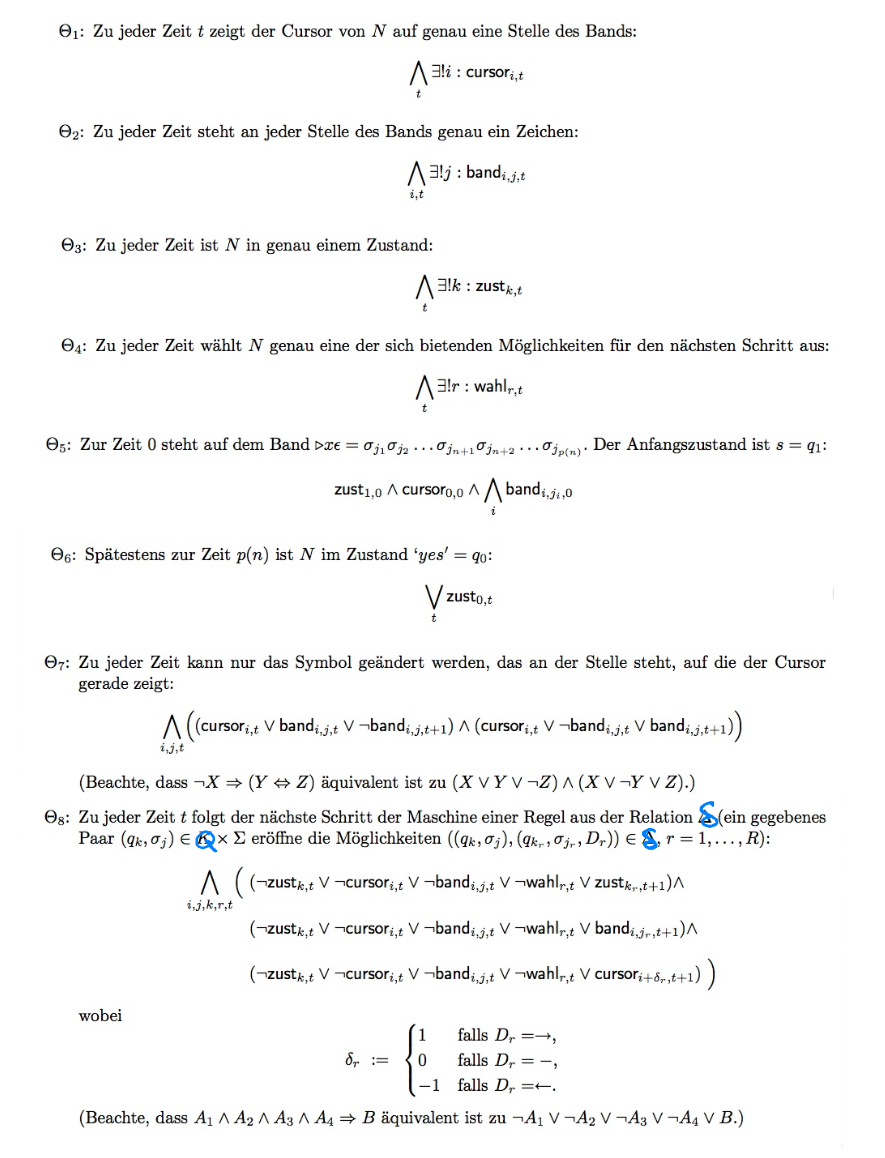
\includegraphics[width=\textwidth]{./SATSchreibweisen}

Man kann sich davon überzeugen, dass es genau dann eine Belegung der Variablen gibt, die alle Klauseln erfüllt, wenn $N$ mit Eingabe $x$ in einen akzeptierenden Endzustand gelangen kann. $\hfill \square$

\subparagraph{Lemma} Ist $L_2 \in NP$ und $L_1$ NP- vollständig und $L_1 \leq_p L_2$, so ist $L_2$ NP- vollständig.
\subparagraph{Beweis} Transititvität von $\leq_p \hfill \square$

\subparagraph{Satz} SAT $\leq_p$ CLIQUE
\subparagraph{Korollar} CLIQUE ist NP- vollständig.



\newpage
\section{Anhang}
\subsection{Grundbegriffe}
\paragraph*{Computer}
\begin{itemize}
\item Maschine, die geistige Routinearbeiten durchführt
\item führt einfache Operationen mit hoher Geschwindigkeit aus
\item $\Rightarrow$ Arbeit muss in Basisoperationen zerlegt werden und dem Rechner mitgeteilt werden (Algorithmus)
\end{itemize}
\paragraph*{Algorithmus}
\begin{itemize}
\item präzise
\item endlich
\item enthält ausführbare elementare Arbeitsschritte
\end{itemize}
\paragraph*{Prozess}
\begin{itemize}
\item Ausführung eines Algorithmus'
\item besitzt stets einen Zustand, der den aktuellen Stand der Ausführung angibt
\end{itemize}
\paragraph*{Prozessor}
\begin{itemize}
\item führt den Prozess aus
\item kann Mensch oder Maschine sein
\end{itemize}
\subsection{Pseudocode}
Präzise, sprachunabhängige Beschreibung von Algorithmen.\\
Keine sprach- spezifische Syntax, keine Typdeklarationen, keine Effizienz- Tricks\\
\\
\textbf{Grundform:}\\\\
\textbf{\emph{Algorithmenname (Parameterliste)\\}}
\textbf{Input:\\
Output:\\}
Programmschritte\\

\paragraph*{Befehle}
\begin{tabular}{c c c}

Bedeutung & Pseudocode & Java\\
\hline
Zuweisung & := & = \\
Vergleich & =, $\neq$, $\leq$, $\geq$, <, > & ==, !=, <=, >=, <, >\\
Logisches UND & AND, $\land$ & \&\&\\
Logisches Oder & OR, $\lor$ & || \\
Logisches Nicht & NOT, $\neg$ & ! \\
Kommentar & // & //, /* */ \\
Rückgabe & RETURN & return\\
\end{tabular}

\paragraph*{Besondere Anweisungen:}
\subparagraph{Verzweigung} $ $\\
IF (condition) THEN\\
\hspace*{2em} ...\\
ELSE IF (condition2) THEN\\
\hspace*{2em} ...\\
ELSE
\hspace*{2em} ...\\
ENDIF

 \begin{lstlisting}
if (condition) {
} else if (condition2) {
} else {
}
\end{lstlisting}

\subparagraph{For- Schleife} $ $\\
FOR i := 1 TO n DO\\
\hspace*{2em} ... \\
ENDFOR \\\\
FORALL $a \in A$ DO \\
\hspace*{2em} ... \\
ENDFOR

\begin{lstlisting}
for (int i = 1; i <=n; i = i+1) {

}

for (Datentyp a : A) {

}
\end{lstlisting}

\subparagraph{While- Schleife}
WHILE (condition) DO\\
\hspace*{2em} ... \\
ENDWHILE \\\\
DO \\
\hspace*{2em} ... \\
WHILE (condition)

\begin{lstlisting}
while (condition) {


do {

} while (condition);
\end{lstlisting}



\subsection{Beweis der Richtigkeit von Algorithmen}
Erfolgt, v.a. bei Rekursion, mit Induktion.
Gerne werden dazu Schleifeninvarianten verwendet.
Alternativ dazu gibt es Widerspruchsbeweise.

\subsubsection {Terminologie}
\paragraph{partielle Korrektheit} Liefert das korrekte Ergebnis bei Terminieren.
\paragraph{Terminieren} Der Algorithmus läuft in keinem Fall unendlich lange ("Endlosschleife" o.ä.), sondern ist nach einer endlichen Zeit abgearbeitet.
\paragraph{totale Korrektheit} Ist partiell korrekt und terminiert immer.

\subsubsection{Schleifeninvariante}
Ist eine Eigenschaft einer Schleife in einem Algorithmus, die zu einem bestimmten Zeitpunkt in jedem Schleifendurchlauf gültig ist.

\subsubsection{Widerspruchsbeweis}
Heißt auch indirekter Beweis oder reductio ad absurdum. Folgendes Vorgehen:
\begin{itemize}
\item Nimm das logisches Gegenteil dessen an, was bewiesen werden soll (Widerspruchsannahme).
\item Mit Widerspruchsannahme und den Voraussetzungen der Behauptung schlussfolgern.
\item Widerspruch herleiten
\item Fertig.
\end{itemize}


\newpage
\subsection{Laufzeitanalyse}
A priori (Rechnerunabhängig, s.u.) oder A posteriori (empirisch getestet)


\paragraph*{Worst-Case Komplexität:} Obere Schranke für die Ausführungszeit in Form der Anzahl auszuführender Operationen in Abhängigkeit von der Größe des Inputs, gemessen in relevanten Parametern (z.B. Anzahl der zu sortierenden Objekte, Stellenzahl von Zahlen, etc.)
\paragraph*{Mittlere Komplexizität:} Obere Schranke für die mittlere Ausführungszeit bei gewissen (Wahrscheinlichkeits-) Annahmen über das Auftreten der Problemdaten
\paragraph*{Untere Komplexizitätsschranken:} Untere Schranken für die (worst-case oder mittlere) Ausführungszeit.\\

Im Idealfall liegen obere und untere Schranke nah beieinander, das ist in der Praxis jedoch nur schwer zu erreichen.

\subsubsection{Asymptotische Notation}
Sei $g: \mathbb{N} \rightarrow \mathbb{N}$. Dann bezeichnet man
\[O(g) := \{ f: \mathbb{N} \rightarrow \mathbb{N} | \exists \, c > 0 \quad und \quad \exists \, n_0 \in \mathbb{N} \quad mit \quad f(n) \leq c \cdot g(n) \,  \forall \, n \geq n_0 \}\]
Liegt eine Funktion $ f: \mathbb{N} \rightarrow \mathbb{N} $ zu dieser Menge, so schreibt man $f \in O(g(n))$.\\
\\
Für eine Polynomfunktion $f(n) = a_m \cdot n^{m} + a_{m-1} \cdot n^{(m-1)} + ... + a_1 n + a_0 $ mit $a_m \neq 0$ gilt $f \in O(n^{m}).$\\

Terme kleiner Ordnung sowie Konstanten werden vernachlässigt, weil bei großen n allein die Größenordnung ausschlaggebend ist und Konstanten und Terme niedriger Ordnung teils auch von der Maschine oder Programmiersprache abhängig sind.\\

\newpage
\subsubsection{Unterscheidung von Größenordnungen}
Erfolgt per o- Notation:
\[o(g) := \{f : \mathbb{N} \rightarrow \mathbb{N} | \forall c > 0 \, \exists \, n_0 \in \mathbb{N} \,\, mit \,\, f(n) < c \cdot g(n) \, \forall n \geq n_0\} \]
$f \in o(g) \Leftrightarrow $ f ist von (echt) kleinerer Größenordnung als g.

Es gilt: $O (f(n)) < O (g(n)) : \Leftrightarrow f(n) \in o(g(n))$

\subsubsection{untere Schranken}
$f \in \Omega (g) : \Leftrightarrow \exists c > 0, \exists n_0 \in \mathbb{N} : f(n) \geq c \cdot g(n) \forall n \geq n_0$

Es gelte $f \in O(g_1) $ und $f \in \Omega (g_2)$.\\
Gilt $g_1 = g_2$, so sagt man $f \in \Theta (g_1)$,\\
d.h. $\Theta (g) := O(g) \cap \Omega (g)$, d.h.
\[f \in \Theta (g) :\Leftrightarrow \exists c_1, c_2 > 0, n_0 \in \mathbb{N}: c_1 \cdot g(n) \leq f(n) \leq c_2 \cdot g(n) \forall n \geq n_0\]\\
\\
Außerdem: $f \in \omega(g) :\Leftrightarrow g \in o(f) \Leftrightarrow \forall c > 0 \exists n_0 \in \mathbb{N} : f(n) > c \cdot g(n) \forall n \geq n_0$

\subsection{Begriffe der Wahrscheinlichkeitstheorie}
\paragraph{(Endlicher Fall)}
\begin{itemize}
\item diskrete Zufallsgröße $X$ 
\item hat Werte $x_1, x_2, ..., x_n$, die mit
\item Wahrscheinlichkeiten $p_1, p_2, ..., p_n$ auftreten.
\item Erwartungswert der Zufallsgröße $X$ ist $E(X) = \sum\limits_{i=1}^{n} x_i \cdot p_i$
\end{itemize}
\paragraph{Abzählbar unendlicher Fall}
\begin{itemize}
\item hat Werte $x_1, x_2, ..., x_i, ...$, mit
\item Wahrscheinlichkeiten $p_1, p_2, ..., p_i, ...$
\item $E(X) = \sum\limits_{i=1}^{\infty} x_i \cdot p_i$, falls Reihe absolut konvergent
\end{itemize}

\subsection{Optimalitätsbeweis des Huffman- Algorithmus'} 
\begin{center}
\includegraphics[width=\textwidth]{./HuffmannLemma1}
\end{center}
\begin{center}
\includegraphics[width=0.95\textwidth]{./HuffmannLemma1B}
\end{center}
\begin{center}
\includegraphics[width=0.95\textwidth]{./HuffmanLemma2}
\end{center}
\begin{center}
\includegraphics[width=\textwidth]{./HuffmannLemma2B}
\end{center}
\begin{center}
\includegraphics[width=\textwidth]{./HuffmannLemma2C}
\end{center}

\newpage
\subsection{Zu BucketSort}
\subsubsection{Beweis der Korrektheit von BucketSort}
Es gilt folgende Invariante: Nach der $i$- ten Iteration sind die Strings nach den letzten $i$ Stellen lexikographisch sortiert.\\\\
\textbf{Beweis per Induktion über $i$}\\
\paragraph{Induktionsanfang}
$i=1$: einfacher BucketSort liefert Behauptung.
\paragraph{Induktionsschluss} Betrachte zwei Fälle
\begin{itemize}
\item [a)] Zwei Strings A und B, die in Iteration $i$ im selben Bucket liegen
\item[b)] A und B in Iteration $i$ in verschiedenen Buckets
\end{itemize}

Zu a)\\
A und B haben dasselbe Zeichen an der $i$- letzten Stelle.

$a_1, ..., a_l, ..., a_k \quad\quad b_1, ..., b_l, ..., b_k \quad\quad l = k + 1 -i$\\
Nach Induktion sind dann A und B lexikographisch sortiert gemäß letzter $i-1$ Zeichen. $\Rightarrow$ Auch lexikographisch korrekt sortiert gemäß letzter $i$ Stellen.

Zu b)\\
A und B haben verschiedene Zeichen an Position $l = k + 1 -i \Rightarrow$ A und B wurden in Iteration $i$ so angeordnet, dass sie lexikographisch sortiert sind gemäß letzter $i$ Zeichen.

$\Rightarrow$ Algorithmus arbeitet korrekt. $\hfill \square$
\subsubsection{Erweiterung von BucketSort zum Sortieren von Strings}
\paragraph{Definition} A, B seien Strings über einem Alphabet (Zeichenmenge $S$). $S$ sei linear geordnet, d.h. $s, t \in S, s \neq t \Rightarrow s < t$ oder $s > t$.
\newpage
\paragraph{Der Algorithmus}
\begin{center}
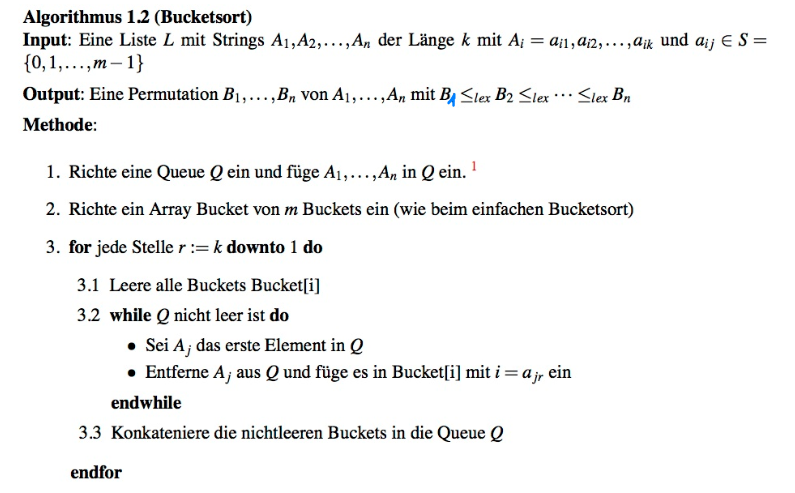
\includegraphics[width=\textwidth]{./BucketsortbeiStrings.png}
\end{center}
\paragraph{Beweis der Korrektheit}
Dann ist $A <_{lex} B$, wenn:
\begin{itemize}
\item A Präfix von B
\item A und B unterscheiden sich an mindestens einer Stelle und an der ersten solchen Stelle gilt: $a_l < b_l$
\end{itemize}
\subparagraph{Spezialfall} Alle Strings haben die gleiche Länge $k$ und $S = \{0, 1\}$
\paragraph{Aufwand}
$k$ mal BucketSort: $O(k(n+m))$

Bei paarweise verschiedenen Binärzahlen: $k \geq \log(n)$

$\rightarrow$ BucketSort bringt nur Vorteile bei vielen identischen Schlüsseln.

\paragraph{Umsetzung}
\subparagraph{Erste Idee} Verwende $k$- stellige Strings mit aufgefüllten kurzen Strings.
\subparagraph{Aufwand} $O(l_{max}(n+m))$
\newpage
\subparagraph{Bessere Variante}
\begin{itemize}
\item[1] Sortiere Strings nach absteigender Länge $O(\underbrace{n} _{< l_{total}} + \underbrace{l_{max}}_{< l_{total}}) \in O(l_{total})$
\item[2] Verwende $l_{max}$- mal einfaches BucketSort, aber betrachte in Iteration $r$ nur die Strings $a_i$, die an der $r$- ten Stelle ein Zeichen haben.
\item[3] Vermeide leere Buckets: Bestimme vorab die benötigten Buckets für jede Iteration und konkateniere dann nur diese.
\end{itemize}
\begin{center}
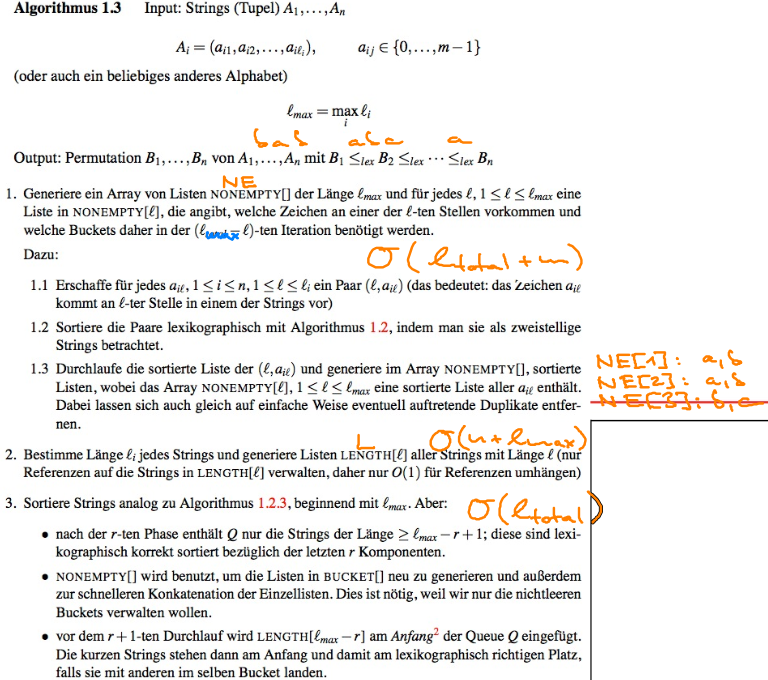
\includegraphics[width=\textwidth]{./BSStringAlgo.png}
\end{center}
\subparagraph{Korrektheit} Folgt aus Korrektheit des allgemeinen BucketSort und der Tatsache, dass die neuen (kurzen) Strings jeweils am Beginn der Liste eingefügt werden.
\subparagraph{Aufwand} Vorbereitung: $O(l_{total}) + O(l_{total} + m)$

\textbf{Sortierphase:} An der Stelle $l$:\\
$n_l$ Strings, $m_l$ Buckets\\
$\rightarrow$ Aufwand $O(\sum\limits_{l=1}^{l_{max}} (n_l + \underbrace{m_l}_{\leq n_l})) = O(\underbrace{\sum\limits_{l=1}^{l_{max}} n_l}_{l_{total}}) = O(l_{total})$

\subsection{Schlussfolgerungen über die Berechenbarkeiten \glqq verwandter\grqq Sprachen}
\subparagraph{Satz} Seien $L, L_1, L_2$ rekursive Sprachen. Dann sind $\bar{L}, L_1 \cup L_2$ und $L_1 \cap$ ebenfalls rekursiv.
\subparagraph{Beweis}
\begin{itemize}
\item[$\bar{L}$] Klar: Vertausche akzeptierende und nichtakzeptierende Endzustände der DTM, die $L$ entscheidet.
\item[$L_1\cup L_2$] Rufe zunächst die DTM auf, die entscheidet, ob Eingabe $x \in L_1$.\\
Falls ja $\rightarrow$ fertig.\\
Falls nein $\rightarrow$ Rufe die DTM auf, die entscheidet, ob $x \in L_2$. Falls ja $\rightarrow$ ja, falls nein $\rightarrow$ nein.

\underline{Alternativer Beweis:} Lasse die beiden DTM für $L_1$ und $L_2$ \glqq parallel\grqq auf einer 2- Band- DTM laufen. Akzeptiere, falls mindestens eine von beiden akzeptiert.
\item[$L_1 \cap L_2$] Wie oben.

\underline{Alternativ:} $L_1 \cap L_2 = \overline{(\overline{L_1} \cup \overline{L_2})}$
\end{itemize} 

\subparagraph{Satz} Seien $L_1, L_2$ rekursiv aufzählbar. Dann sind auch $L_1 \cup L_2$ und $L_1 \cap L_2$ rekursiv aufzählbar.
\subparagraph{Beweis} Nutze Parallelsimulation von oben.

\subparagraph{Lemma} Sind $L$ und $\bar{L}$ rekursiv aufzählbar, so ist $L$ rekursiv.
\subparagraph{Beweis} Parallelsimulation, s.o.

\subparagraph{Satz} Die Menge der rekursiv aufzählbaren Funktionen ist \underline{nicht} abgeschlossen bezüglich Komplementbildung. Insbesondere ist $U$ rekursiv aufzählbar, $\bar{U}$ jedoch nicht.
\subparagraph{Beweis} $U$ ist rekursiv aufzählbar, aber nicht rekursiv.

\subparagraph{Korollar} Für jede Sprache $L$ gibt es genau eine der folgenden 3 Eigenschaften:
\begin{itemize}
\item[1] $L$ und $\bar{L}$ sind rekursiv.
\item[2] $L$ und $\bar{L}$ sind nicht rekursiv aufzählbar.
\item[3] Genau eine der beiden Sprachen $L$ und $\bar{L}$ ist rekursiv aufzählbar (aber nicht rekursiv!)
\end{itemize}



\subsection{Zum Gödel'schen Unvollständigkeitssatz}
\subsubsection{Mathematische Ausdrücke (Sätze)}
\subparagraph{Ein Beispiel}
\[\forall q \in \mathbb{N}_0 \exists p \in \mathbb{N}_0 \forall x, y \in \mathbb{N}_0 (p > q \land (x, y > 1 \Rightarrow (x \cdot y \neq p, x \cdot y \neq p + 2)))\]
\subparagraph{Alphabet} $\Sigma = \{\land, \lor, \neg, (, ), \exists, \forall, x, R_1, ..., R_k \}$\\
$R_1, ..., R_k$ Relationen\\
z.B. Additionsrelation: $R_1(x_i, x_j, x_l) = \glqq wahr\grqq \Leftrightarrow x_i + x_j = x_l$
\subparagraph{Definition} 
Ein Satz ist ein Ausdruck $w \in Sigma^*$ der Form:\\
$Q_1x_1 ... Q_lx_l \Phi$\\
Wobei $Q_1, ..., Q_l \in \{\forall, \exists\}$\\
und die Formel $\Phi$ rekursiv wie folgt definiert ist:
\begin{itemize}
\item[1] $\Phi = R_j(x_{i_1}, x_{i_2},..., x_{i_n})$ für $1 \leq j \leq k, 1 \leq i_r \leq l$ ist Formel.
\item[2] $\Phi = \Phi_1 \land \Phi_2$ oder $\Phi = \Phi_1 \lor \Phi_2$ oder $\Phi = \neq \Phi_1$, wobei $\Phi_1, \Phi_2$ kürzere Formeln sind.
\end{itemize}
\textbf{Ein Satz ist also ein mathematischer Ausdruck, der wahr oder falsch ist.}

\subsubsection{Hilberts Programm}
Baue die Mathematik von Grund auf neu, ausgehend von Axiomen, die konsistent und widerspruchsfrei sein müssen. Die Axiome sollen außerdem vollständig sein, d.h. alles Wahre soll daraus formell abgeleitet werden können.

Gödel zerstörte diesen Traum mit seinem Unvollständigkeitssatz.






\subsection{Sonstiges}
"Überabzählbar unendlich > abzählbar unendlich"


%\cleardoublepage
%\section{Index}
%\renewcommand{\indexname}{Sachverzeichnis}
%\addcontentsline{toc}{section}{Index}
%\printindex
\end{document}